\chapter{\textcolor{azulescom}{Análisis}}

\section{Problemática}

La industria inmobiliaria enfrenta grandes desafíos en la actualidad. La
transformación digital dentro de la industria ha sido lenta, y para los
participantes del mercado, la tecnología disponible no ha sido suficiente para
resolver los problemas que enfrentan. La industria inmobiliaria es una de las
más grandes del mundo, y sin embargo, es una de las que menos ha invertido en
tecnología \cite{pagourtzi2003}.

Para agentes inmobiliarios, compradores, inversionistas y desarrolladores, la
falta de información repercuten en el dinamismo del mercado y limitan la
toma de decisiones. A pesar de que existen plataformas que ofrecen información
sobre el mercado inmobiliario, la información que ofrecen es limitada y no
permite a los participantes del mercado tomar decisiones informadas.

\section{Propuesta de Solución}

La propuesta de solución consiste en desarrollar una plataforma que permita
a los participantes del mercado inmobiliario tomar decisiones informadas,
mediante el análisis de datos de bienes raíces con la finalidad de eficientar
el proceso de estimación de valor de mercado para departamentos en la Ciudad de
México, basado en sus características y ubicación.

Con la finalidad de poder obtener estimaciones de valor de mercado válidas,
se hará uso de técnicas de inteligencia artificial para el entrenamiento de un
modelo de aprendizaje automático que permita predecir el valor de mercado de
departamentos en la Ciudad de México según sus características y ubicación.

A fin de determinar el funcionamiento de la plataforma, se realizará un análisis
exploratorio de datos para determinar la calidad de los datos disponibles para
el entrenamiento del modelo, así como para determinar las características más
relevantes para la predicción del valor de mercado de departamentos en la Ciudad
de México.

\subsection{¿Por qué se eligió emplear Inteligencia Artificial?}

Uno de los aspectos determinantes para realizar valuaciones inmobiliarias válidas
es la precisión con la que se analiza cada inmueble, ya que cada uno de ellos es
único y tiene características que lo hacen diferente a los demás. Por lo tanto,
es necesario contar con un modelo que permita analizar cada inmueble de manera
individual, con el fin de poder obtener estimaciones de valor de mercado válidas.

Analizar cada inmueble de forma individual es una tarea que requiere de mucho
tiempo y esfuerzo, por lo que, empleando las características más distintivas
e impactantes en el valor de mercado de un inmueble, se puede desarrollar un
modelo que permita estimar el valor de mercado de un inmueble de manera rápida
y eficiente.

En contraste con las estrategias tradicionales de valuación inmobiliaria, las
cuales se basan en la comparación de inmuebles similares, el modelo propuesto
se basa en el análisis de las características más distintivas, por lo que los
resultados obtenidos son más precisos y confiables.

Por otro lado, ya que el flujo de información para el entrenamiento del modelo
puede retomarse en distintos puntos del tiempo, es posible realizar actualizaciones
a dicho modelo para que este pueda adaptarse a los cambios en el mercado inmobiliario.

\subsection{¿Por qué se eligió desarrollar una plataforma web?}

Con el objetivo de disponibilizar las conclusiones derivadas del análisis de los
datos y el modelo de aprendizaje automático, se eligió desarrollar un prototipo
de plataforma web que permita a los participantes del mercado inmobiliario
obtener estimaciones de valor de mercado válidas para departamentos en la Ciudad
de México ya que es un medio de fácil acceso y que permite la interacción con
los usuarios de manera sencilla.

La naturaleza del mercado inmobiliario obliga a sus participantes a mantenerse
en movimiento para poder realizar su trabajo, por lo que es necesario que la
plataforma sea accesible desde cualquier dispositivo con acceso a internet.

\section{Herramientas a Emplear}

Para desarrollar la presente propuesta de plataforma se requerirá el uso tanto
de herramientas de software como de hardware. En cuestiones de software, se
considerarán tanto las herramientas destinadas al desarrollo de la plataforma
como las herramientas destinadas al desarrollo del modelo de aprendizaje,
la extracción de datos y la limpieza de los mismos. En cuestiones de hardware,
se considerarán los equipos con los que se disponen para realizar el desarrollo
del proyecto.

\subsection{Herramientas de Software}

En esta sección se hará mención de las herramientas de software, lenguajes y
librerías más importantes que se emplearán para el desarrollo de la plataforma.

\subsubsection{Python}

Python es un lenguaje de programación \textit{multi-paradigma} que brinda completo
soporte a la programación orientada a objetos y a la programación estructurada,
además de contar con diversas características que apoyan la programación funcional
y la programación orientada a aspectos, incluyendo metaprogramación y
\textit{métodos mágicos}. Python utiliza \textit{tipado dinámico} y una
combinación de \textit{conteo de referencias} junto con un
\textit{recolector de basura detector de ciclos} para la gestión de memoria.
Una característica importante de Python es la \textit{resolución dinámica de nombres}
(\textit{late binding}), que vincula nombres de métodos y variables durante la
ejecución del programa. A pesar de ofrecer solo un soporte limitado para la
programación funcional al estilo de Lisp, el lenguaje incluye funciones como
\texttt{map()}, \texttt{reduce()} y \texttt{filter()}, comprensiones para listas,
diccionarios y conjuntos, así como expresiones generadoras. Su filosofía se centra
en la simplicidad y la legibilidad, rechazando la sintaxis exuberante a favor de
una gramática más clara y menos recargada. Los desarrolladores de Python buscan
evitar la \textit{optimización prematura} y rechazan cambios en partes no críticas
de CPython que ofrezcan un aumento marginal en velocidad a costa de la claridad.
Un objetivo importante de los desarrolladores de Python es hacer que el lenguaje
sea \textit{divertido de usar}, lo que se refleja en el origen del nombre y en
un enfoque ocasionalmente lúdico hacia tutoriales y materiales de referencia
\cite{van2007python}.

Algunas ventajas de utilizar Python son:

\begin{itemize}
  \item Es un lenguaje de programación de alto nivel, lo que permite escribir
  programas más cortos y fáciles de leer.
  \item Es un lenguaje de programación interpretado, lo que permite ejecutar
  programas sin necesidad de compilarlos.
  \item Es un lenguaje de programación multiparadigma, lo que permite utilizar
  distintos estilos de programación.
  \item Es un lenguaje de programación multiplataforma, lo que permite ejecutar
  programas en distintos sistemas operativos.
  \item Es un lenguaje de programación orientado a objetos, lo que permite
  reutilizar código y crear programas modulares.
  \item Es un lenguaje de programación extensible, lo que permite agregar
  funcionalidades mediante el uso de módulos.
\end{itemize}

Por otro lado, algunas desventajas de utilizar Python son:

\begin{itemize}
  \item Es un lenguaje de programación interpretado, lo que hace que los
  programas sean más lentos que los programas escritos en lenguajes compilados.
  \item Es un lenguaje de programación de alto nivel, lo que hace que los
  programas sean más lentos que los programas escritos en lenguajes de bajo nivel.
\end{itemize}

\subsubsection{Pandas}

\texttt{pandas} es un paquete de Python que proporciona estructuras de datos
rápidas, flexibles y expresivas diseñadas para facilitar y hacer intuitivo el
trabajo con datos ``relacionales'' o ``etiquetados''. Su objetivo es ser el
bloque de construcción fundamental de alto nivel para realizar análisis de datos
prácticos y reales en Python. Además, tiene el objetivo más amplio de convertirse
en la herramienta de análisis y manipulación de datos de código abierto más
poderosa y flexible disponible en cualquier lenguaje. Ya está bien encaminado
hacia este objetivo \cite{mckinney2011pandas}.

\texttt{pandas} es adecuado para muchos tipos diferentes de datos:

\begin{itemize}
    \item Datos tabulares con columnas de tipos heterogéneos, como en una tabla
      SQL o una hoja de cálculo Excel.
    \item Datos de series temporales ordenados y no ordenados (no necesariamente
      de frecuencia fija).
    \item Datos de matriz arbitrarios (tipados homogéneamente o heterogéneos)
      con etiquetas de filas y columnas.
    \item Cualquier otra forma de conjuntos de datos observacionales/estadísticos.
      Los datos no necesitan estar etiquetados para ser colocados en una estructura
      de datos de \texttt{pandas}.
\end{itemize}

Se ha elegido \texttt{pandas} debido a que es una herramienta de análisis de
datos de alto rendimiento y fácil de usar, la cual permite realizar análisis
exploratorios de datos de manera sencilla.

\subsubsection{NumPy}

\texttt{NumPy} es el paquete fundamental para la computación científica en Python.
Es una biblioteca de Python que proporciona un objeto de arreglo multidimensional,
varios objetos derivados (como arreglos enmascarados y matrices) y una variedad de
rutinas para operaciones rápidas en arreglos, incluyendo operaciones matemáticas,
lógicas, manipulación de formas, ordenamiento, selección, E/S, transformadas de
Fourier discretas, álgebra lineal básica, operaciones estadísticas básicas,
simulación aleatoria y mucho más \cite{oliphant2006guide}.

Se ha elegido \texttt{NumPy} debido a que ofrece una gran cantidad de funciones
matemáticas que resultan útiles (y necesarias) para la realización de un
análisis exploratorio de datos válido.

\subsubsection{StatsModels}

\texttt{Statsmodels} es una biblioteca para análisis estadístico y econométrico
en Python, dirigida tanto a estadísticos y economistas teóricos y aplicados,
como a usuarios y desarrolladores de Python de distintas disciplinas que utilizan
modelos estadísticos. Es especialmente útil para aquellos usuarios de R, Stata,
SAS, SPSS, NLOGIT, GAUSS o MATLAB interesados en trabajar en Python por sus beneficios.
Inicialmente parte de SciPy como \texttt{models}, luego se integró en el proyecto
de neuroimagen NIPY para su maduración y evolución. Mejorado durante el
Google Summer of Code 2009 y 2010, ahora se distribuye como un SciKit, o paquete
adicional para SciPy. Sus principales desarrolladores, formados en economía y
con experiencia en econometría, han enfocado su desarrollo en aplicaciones
econométricas, aunque su diseño busca ser amigable y extensible por desarrolladores
de cualquier disciplina. El trabajo continuo está ampliando su utilidad para
necesidades comunes de modelado estadístico \cite{seabold2010statsmodels}.

Esta librería se ha elegido ya que es idónea para realizar el análisis exploratorio
econométrico con el cual determinaremos los factores más relevantes para la
predicción del valor de mercado de departamentos en la Ciudad de México, así como
establecer los criterios apropiados para la elección del modelo de aprendizaje
automático.

\subsubsection{Scikit-Learn}

Scikit-learn es un módulo de Python que integra una amplia gama de algoritmos
de aprendizaje automático de última generación para problemas supervisados y no
supervisados de escala media. Este paquete se centra en llevar el aprendizaje
automático a los no especialistas utilizando un lenguaje de alto nivel de propósito
general. Se pone énfasis en la facilidad de uso, el rendimiento, la documentación
y la consistencia de la API. Tiene dependencias mínimas y se distribuye bajo la
licencia BSD simplificada, fomentando su uso tanto en entornos académicos como
comerciales \cite{pedregosa2011scikit}.

Se ha elegido \texttt{Scikit-Learn} debido a que es una herramienta de aprendizaje
automático sencilla de usar, la cual permite entrenar modelos de aprendizaje
automático de manera sencilla y, para fines de este proyecto, permite realizar
análisis de componentes principales y regresión simple y múltiple.

\subsubsection{TensorFlow}

TensorFlow es un sistema de aprendizaje automático que opera a gran escala y en
entornos heterogéneos. Su modelo computacional se basa en grafos de flujo de
datos con estado mutable. Los nodos del grafo pueden mapearse a diferentes
máquinas en un clúster, y dentro de cada máquina a CPUs, GPUs y otros
dispositivos. TensorFlow admite una variedad de aplicaciones, pero se enfoca
particularmente en el entrenamiento y la inferencia con redes neuronales
profundas. Sirve como plataforma tanto para la investigación como para la
implementación de sistemas de aprendizaje automático en muchas áreas, tales
como reconocimiento de voz, visión por computadora, robótica, recuperación de
información y procesamiento de lenguaje natural. En esta charla, describimos
TensorFlow y esbozamos algunas de sus aplicaciones. También discutimos la
cuestión de qué relación puede tener TensorFlow y el aprendizaje profundo con
la programación funcional. Aunque TensorFlow no es puramente funcional, muchos
de sus usos están relacionados con la optimización de funciones (durante el
entrenamiento), y luego con la aplicación de esas funciones (durante la
inferencia). Estas funciones se definen como composiciones de primitivas
simples (como es común en la programación funcional), con representaciones
internas de datos que se aprenden en lugar de diseñarse manualmente. TensorFlow
es un trabajo conjunto con muchas otras personas del equipo de Google Brain y
otros lugares \cite{abadi2016tensorflow}.

Se ha elegido \texttt{TensorFlow} debido a que es una herramienta de aprendizaje
automático que permite entrenar modelos de aprendizaje automático de manera
sencilla y, para fines de este proyecto, permite entrenar modelos de aprendizaje
automático de regresión, además de integrarse directamente con FastAPI.

\subsubsection{FastAPI}

FastAPI es un moderno marco de trabajo web de API de Python de alto rendimiento, basado en
OpenAPI (anteriormente conocido como Swagger) y estándares de tipo de datos
estándar de Python. El marco es ideal para crear microservicios rápidos y
escalables, ya que es fácil de aprender y usar, y ofrece una gran cantidad de
características útiles, como la generación automática de documentación,
validación de datos, pruebas unitarias y de integración, y mucho más \cite{voron2023building}.

Se ha elegido \texttt{FastAPI} debido a que es un marco de trabajo web de API
que permite desarrollar APIs de manera sencilla y rápida, además de integrarse
directamente con TensorFlow.

\subsubsection{QGIS}
QGIS es un sistema de información geográfica (SIG) de código abierto que comenzó
en 2002 y opera en plataformas Unix, Windows y macOS. Desarrollado con Qt y C++,
ofrece una interfaz de usuario amigable, además de aplicaciones para dispositivos
móviles. Inicialmente un visor de datos SIG, ahora QGIS es utilizado para
visualización de datos GIS, captura de datos, análisis avanzado y presentaciones
en mapas. Admite numerosos formatos de datos y se expande fácilmente con complementos.
Publicado bajo la Licencia Pública General GNU (GPL), QGIS es gratuito y de código
fuente abierto, asegurando acceso y modificación libres \cite{qgis_3.28_user_guide}.

Se ha elegido usar QGIS debido a que es un software de código abierto que permite
realizar análisis geoespaciales de manera sencilla y rápida, además de que permite
visualizar los datos de manera sencilla. En la Figura \ref{fig:qgis} se muestra
una captura de pantalla de QGIS con los datos de bienes raíces de la Ciudad de
México.

\begin{figure}[H]
  \centering
  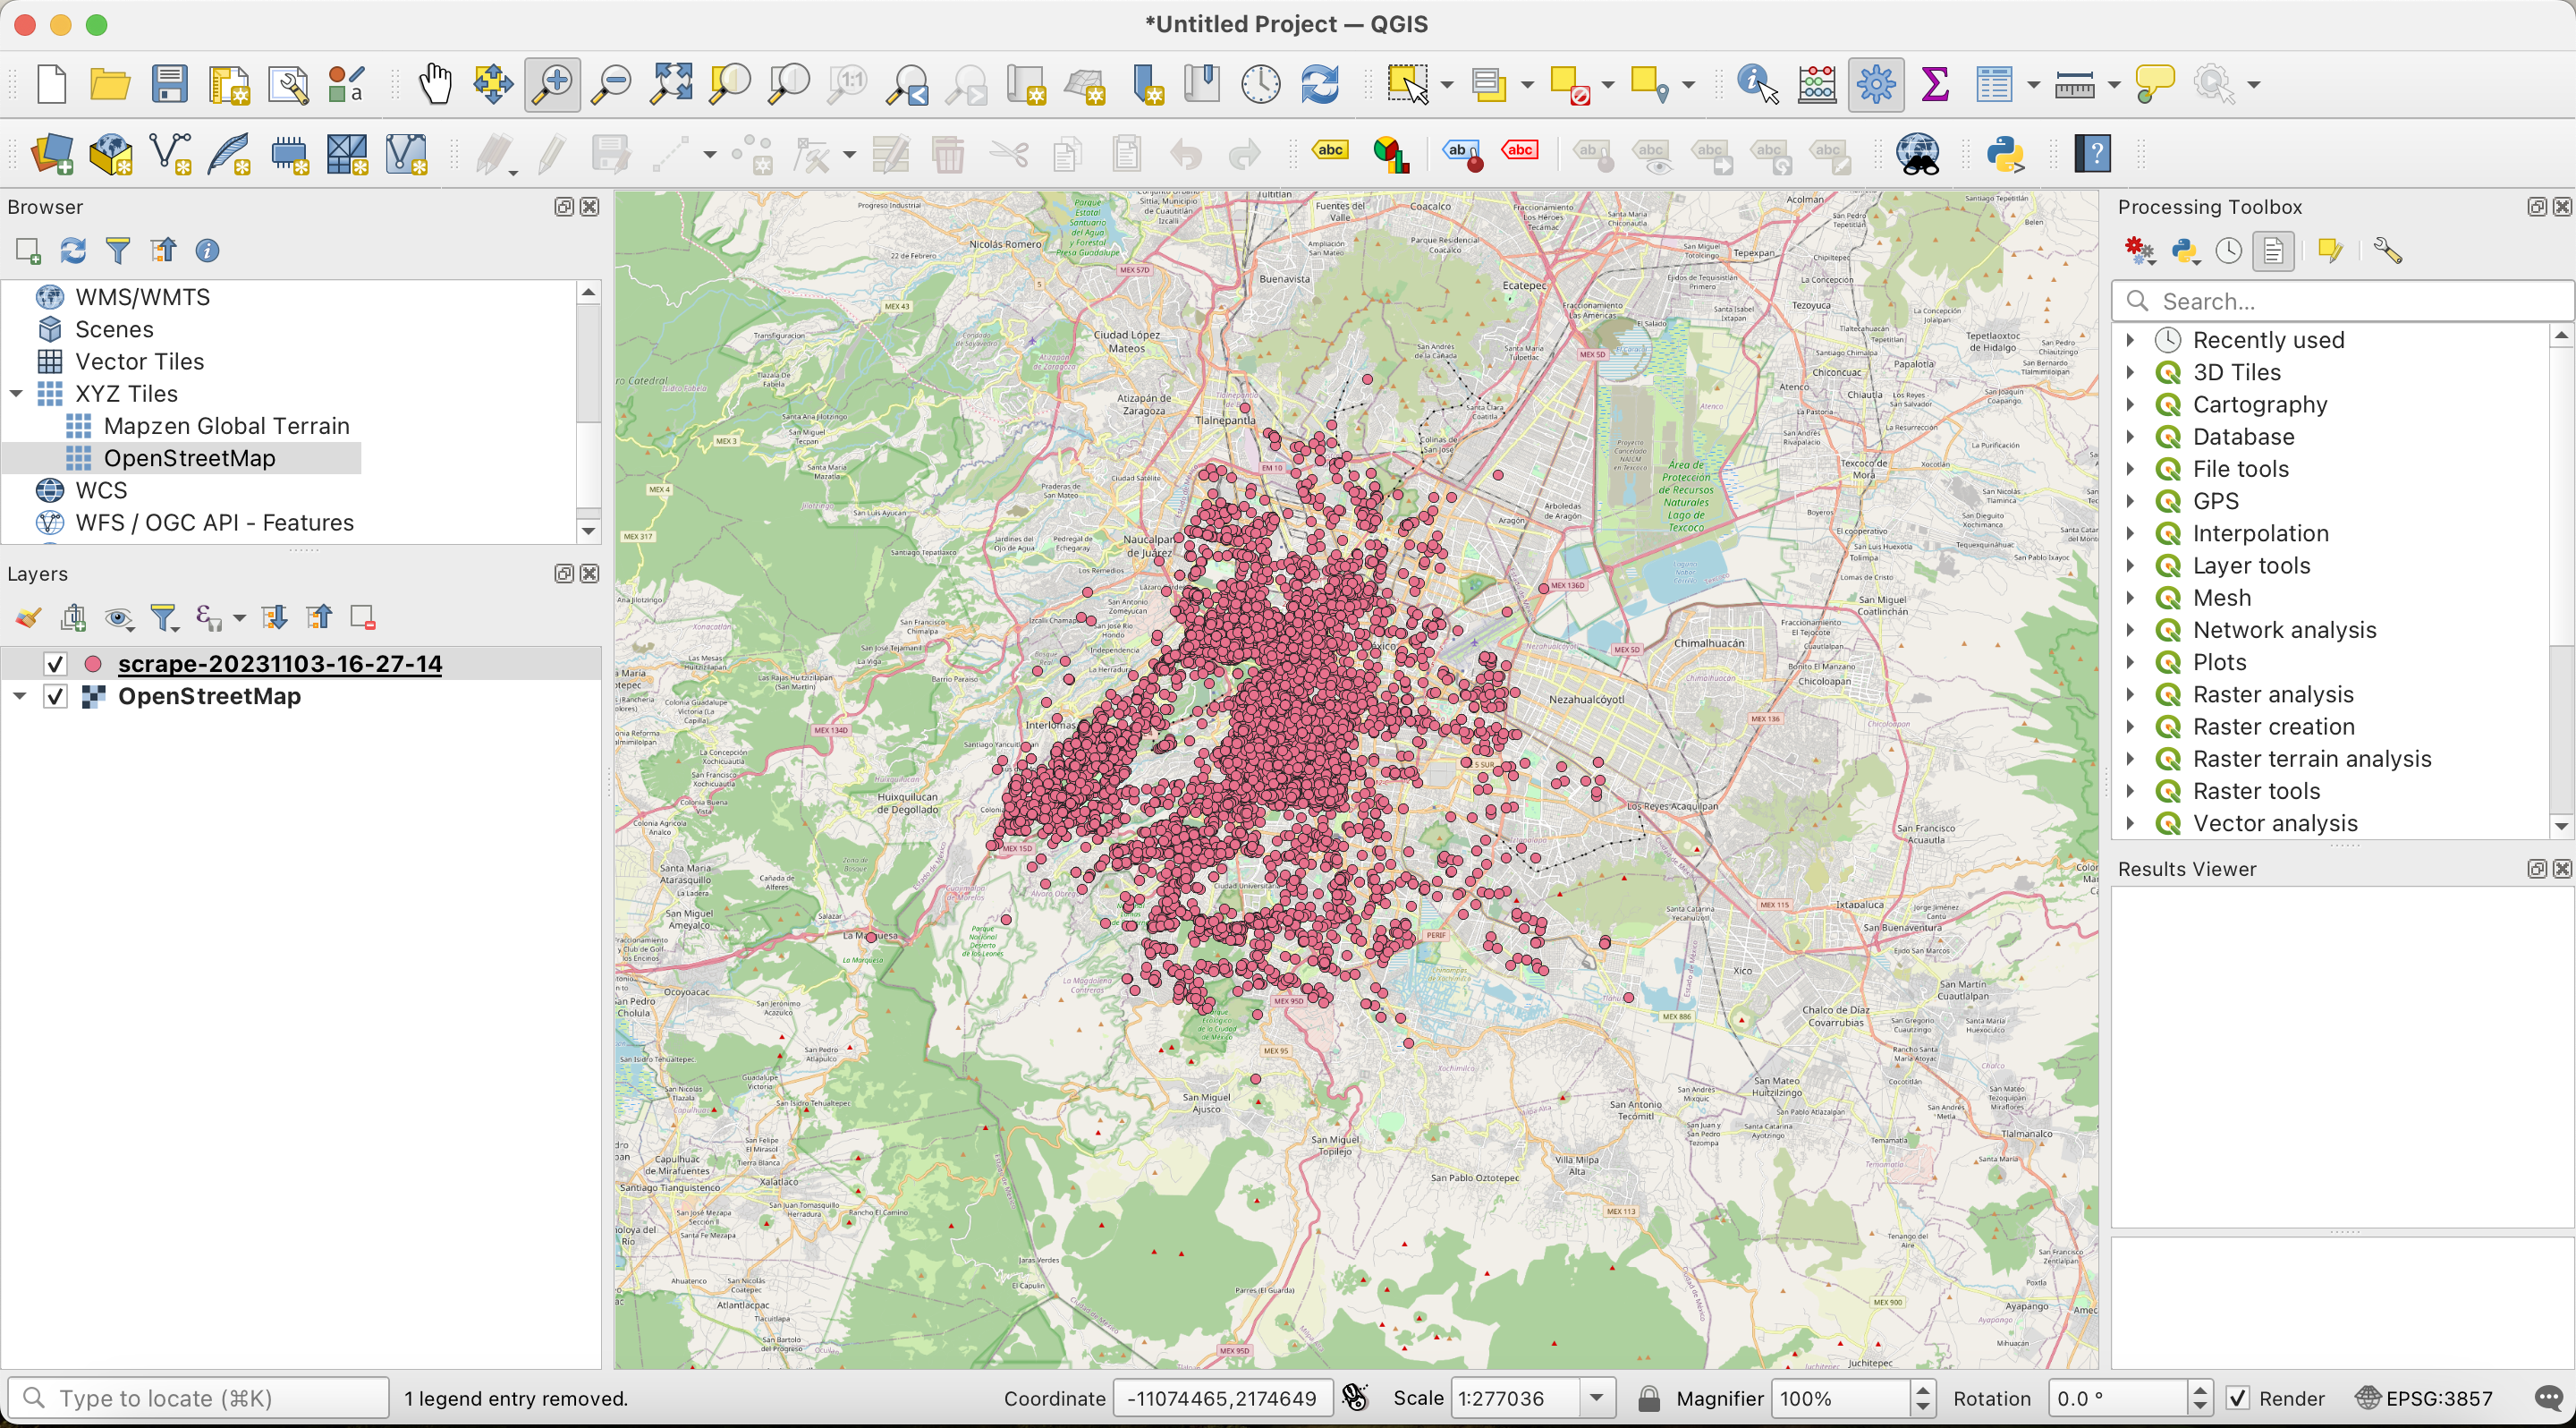
\includegraphics[width=0.9\textwidth]{imagenes/03-analisis/captura-qgis.png}
  \caption{Captura de pantalla de QGIS con los datos de bienes raíces de la Ciudad de México.}
  \label{fig:qgis}
\end{figure}

\subsubsection{React}
React es un marco de trabajo de código abierto desarrollado por Facebook para
crear interfaces de usuario. Se utiliza para manejar la capa de vista para aplicaciones
web y móviles. Una de las principales características de React es que utiliza
un enfoque basado en componentes para el desarrollo de aplicaciones. Con React,
los desarrolladores pueden crear componentes reutilizables que se pueden utilizar
para crear interfaces de usuario complejas. React también permite a los desarrolladores
crear interfaces de usuario declarativas. Esto significa que los desarrolladores
pueden escribir código que describa cómo debería ser la interfaz de usuario.
React se encarga de actualizar automáticamente la interfaz de usuario cuando
los datos cambian, lo que permite a los desarrolladores evitar tener que
escribir código adicional para actualizar la interfaz de usuario \cite{ReactLearn2023}.

Se eligió React debido a que es un marco de trabajo conocido por el equipo de
desarrollo, además de que, al ser de código abierto y alta popularidad, goza de
una gran cantidad de documentación, soporte y librerías que facilitan el desarrollo
de aplicaciones web.

\subsubsection{Material-UI}
Material-UI es una biblioteca de componentes de interfaz de usuario para React
que implementa el lenguaje de diseño de Google, Material Design, para la web.
Material-UI hace que el desarrollo de aplicaciones web sea más rápido y fácil \cite{mui_getting_started}.

Se decidió trabajar con Material-UI debido a que su implementación es conocida
por el equipo de desarrollo y su diseño es atractivo y moderno.

\subsubsection{Docker}
Docker es un proyecto de código abierto que automatiza el despliegue de aplicaciones
dentro de contenedores de software, proporcionando una capa adicional de abstracción
y automatización de virtualización de aplicaciones en múltiples sistemas operativos.
Docker utiliza características de aislamiento de recursos del kernel de Linux, como
cgroups y espacios de nombres (namespaces) para permitir que ``contenedores'' independientes
se ejecuten dentro de una sola instancia de Linux, evitando la sobrecarga de iniciar y
mantener máquinas virtuales (VMs) \cite{docker_overview}.

Se eligió Docker para empaquetar la aplicación web y facilitar su despliegue en
cualquier servidor, en nuestro caso, en la nube.

\subsection{Herramientas de Hardware}

En tanto a hardware se refiere, para el desarrollo de este proyecto se empleará
una computadora portátil con las siguientes características:

\begin{itemize}
  \item Procesador Apple M1 de 8 núcleos, 4 de rendimiento y 4 de eficiencia.
  \item GPU de 8 núcleos.
  \item 8 GB de memoria unificada.
  \item 256 GB de almacenamiento SSD.
  \item Pantalla Retina de 13 pulgadas con tecnología True Tone.
  \item Touch Bar y Touch ID.
  \item Dos puertos Thunderbolt / USB 4.
\end{itemize}

\subsubsection{Amazon Web Services}

Debido a que se pretende que la aplicación web sea accesible desde cualquier
dispositivo con acceso a internet, se consideró la posibilidad de emplear
servicios de computación en la nube para el despliegue de la aplicación web.
De los servicios de computación en la nube disponibles, se eligió Amazon Web
Services (AWS) debido a que es el servicio de computación en la nube más
popular y cuenta con una gran cantidad de documentación, soporte y librerías
que facilitan el despliegue de aplicaciones web.

Aunque el entrenamiento de los modelos de aprendizaje automático se realizará
en la computadora portátil mencionada anteriormente, el despliegue del sistema
final se realizará en un servicio de computación en la nube.

\section{Análisis Exploratorio de Datos}

El análisis exploratorio de datos es una parte fundamental del proceso de
minería de datos, ya que permite obtener información relevante sobre los datos
que se utilizarán para el entrenamiento del modelo de aprendizaje automático.
A su vez, permite identificar patrones, tendencias y
relaciones entre los datos, lo cual permite determinar la calidad de los datos
y la relevancia de las variables para el entrenamiento del modelo \cite{stephan2009exploratory}.

Debido a la naturaleza del proyecto, los datos que se utilizarán para el
entrenamiento del modelo de aprendizaje automático son datos de bienes raíces
georeferenciados mediante una latitud y longitud, por lo que el análisis
consistirá en un análisis exploratorio geoespacial y un análisis exploratorio
econométrico.

El conjunto de datos empleado para el análisis exploratorio de datos es un
conjunto de datos de bienes raíces de la Ciudad de México, el cual fue obtenido
de la plataforma Inmuebles24 \cite{inmuebles24}. Este conjunto de datos contiene
información sobre 40,000 anuncios de bienes raíces de la Ciudad de México,
los cuales fueron publicados hasta el 30 de Agosto de 2023. El conjunto de datos
se obtuvo únicamente para, a partir del presente análisis exploratorio de datos,
determinar la calidad de los datos y la relevancia de las variables para el
entrenamiento del modelo de aprendizaje automático. Para el desarrollo de la
plataforma final, se utilizará un conjunto de datos que incorpore los datos
extraídos durante el desarrollo del proyecto a bien de tener un conjunto de
datos más completo y actualizado.

\subsection{Análisis Exploratorio Geoespacial}

Como se mencionó, los datos tienen una componente geoespacial, por lo que es
importante realizar un análisis exploratorio geoespacial para poder obtener
información relevante. Dentro de este análisis se realizarán los siguientes
análisis:

\begin{itemize}
  \item Visualización de puntos de anuncios
  \item Mapa de densidad de anuncios por alcaldía
  \item Mapa de calor de precios
  \item Mapa de calor de número de recámaras
  \item Mapa de calor de número de baños
  \item Mapa de calor de metros cuadrados
  \item Mapa de calor de antigüedad
  \item Mapa de calor de estacionamientos
\end{itemize}

\subsubsection{Visualización de puntos de anuncios}

La visualización de puntos de anuncios permite representar individualmente cada
anuncio. Esto permite realizar un análisis de distribución geográfica y relación
con puntos de interés (parques, escuelas, centros comerciales, etc.). En la
Figura \ref{fig:visualizacion_puntos_anuncios} se muestra la visualización de
puntos de anuncios para el conjunto de datos de bienes raíces.

\begin{figure}[H]
  \centering
  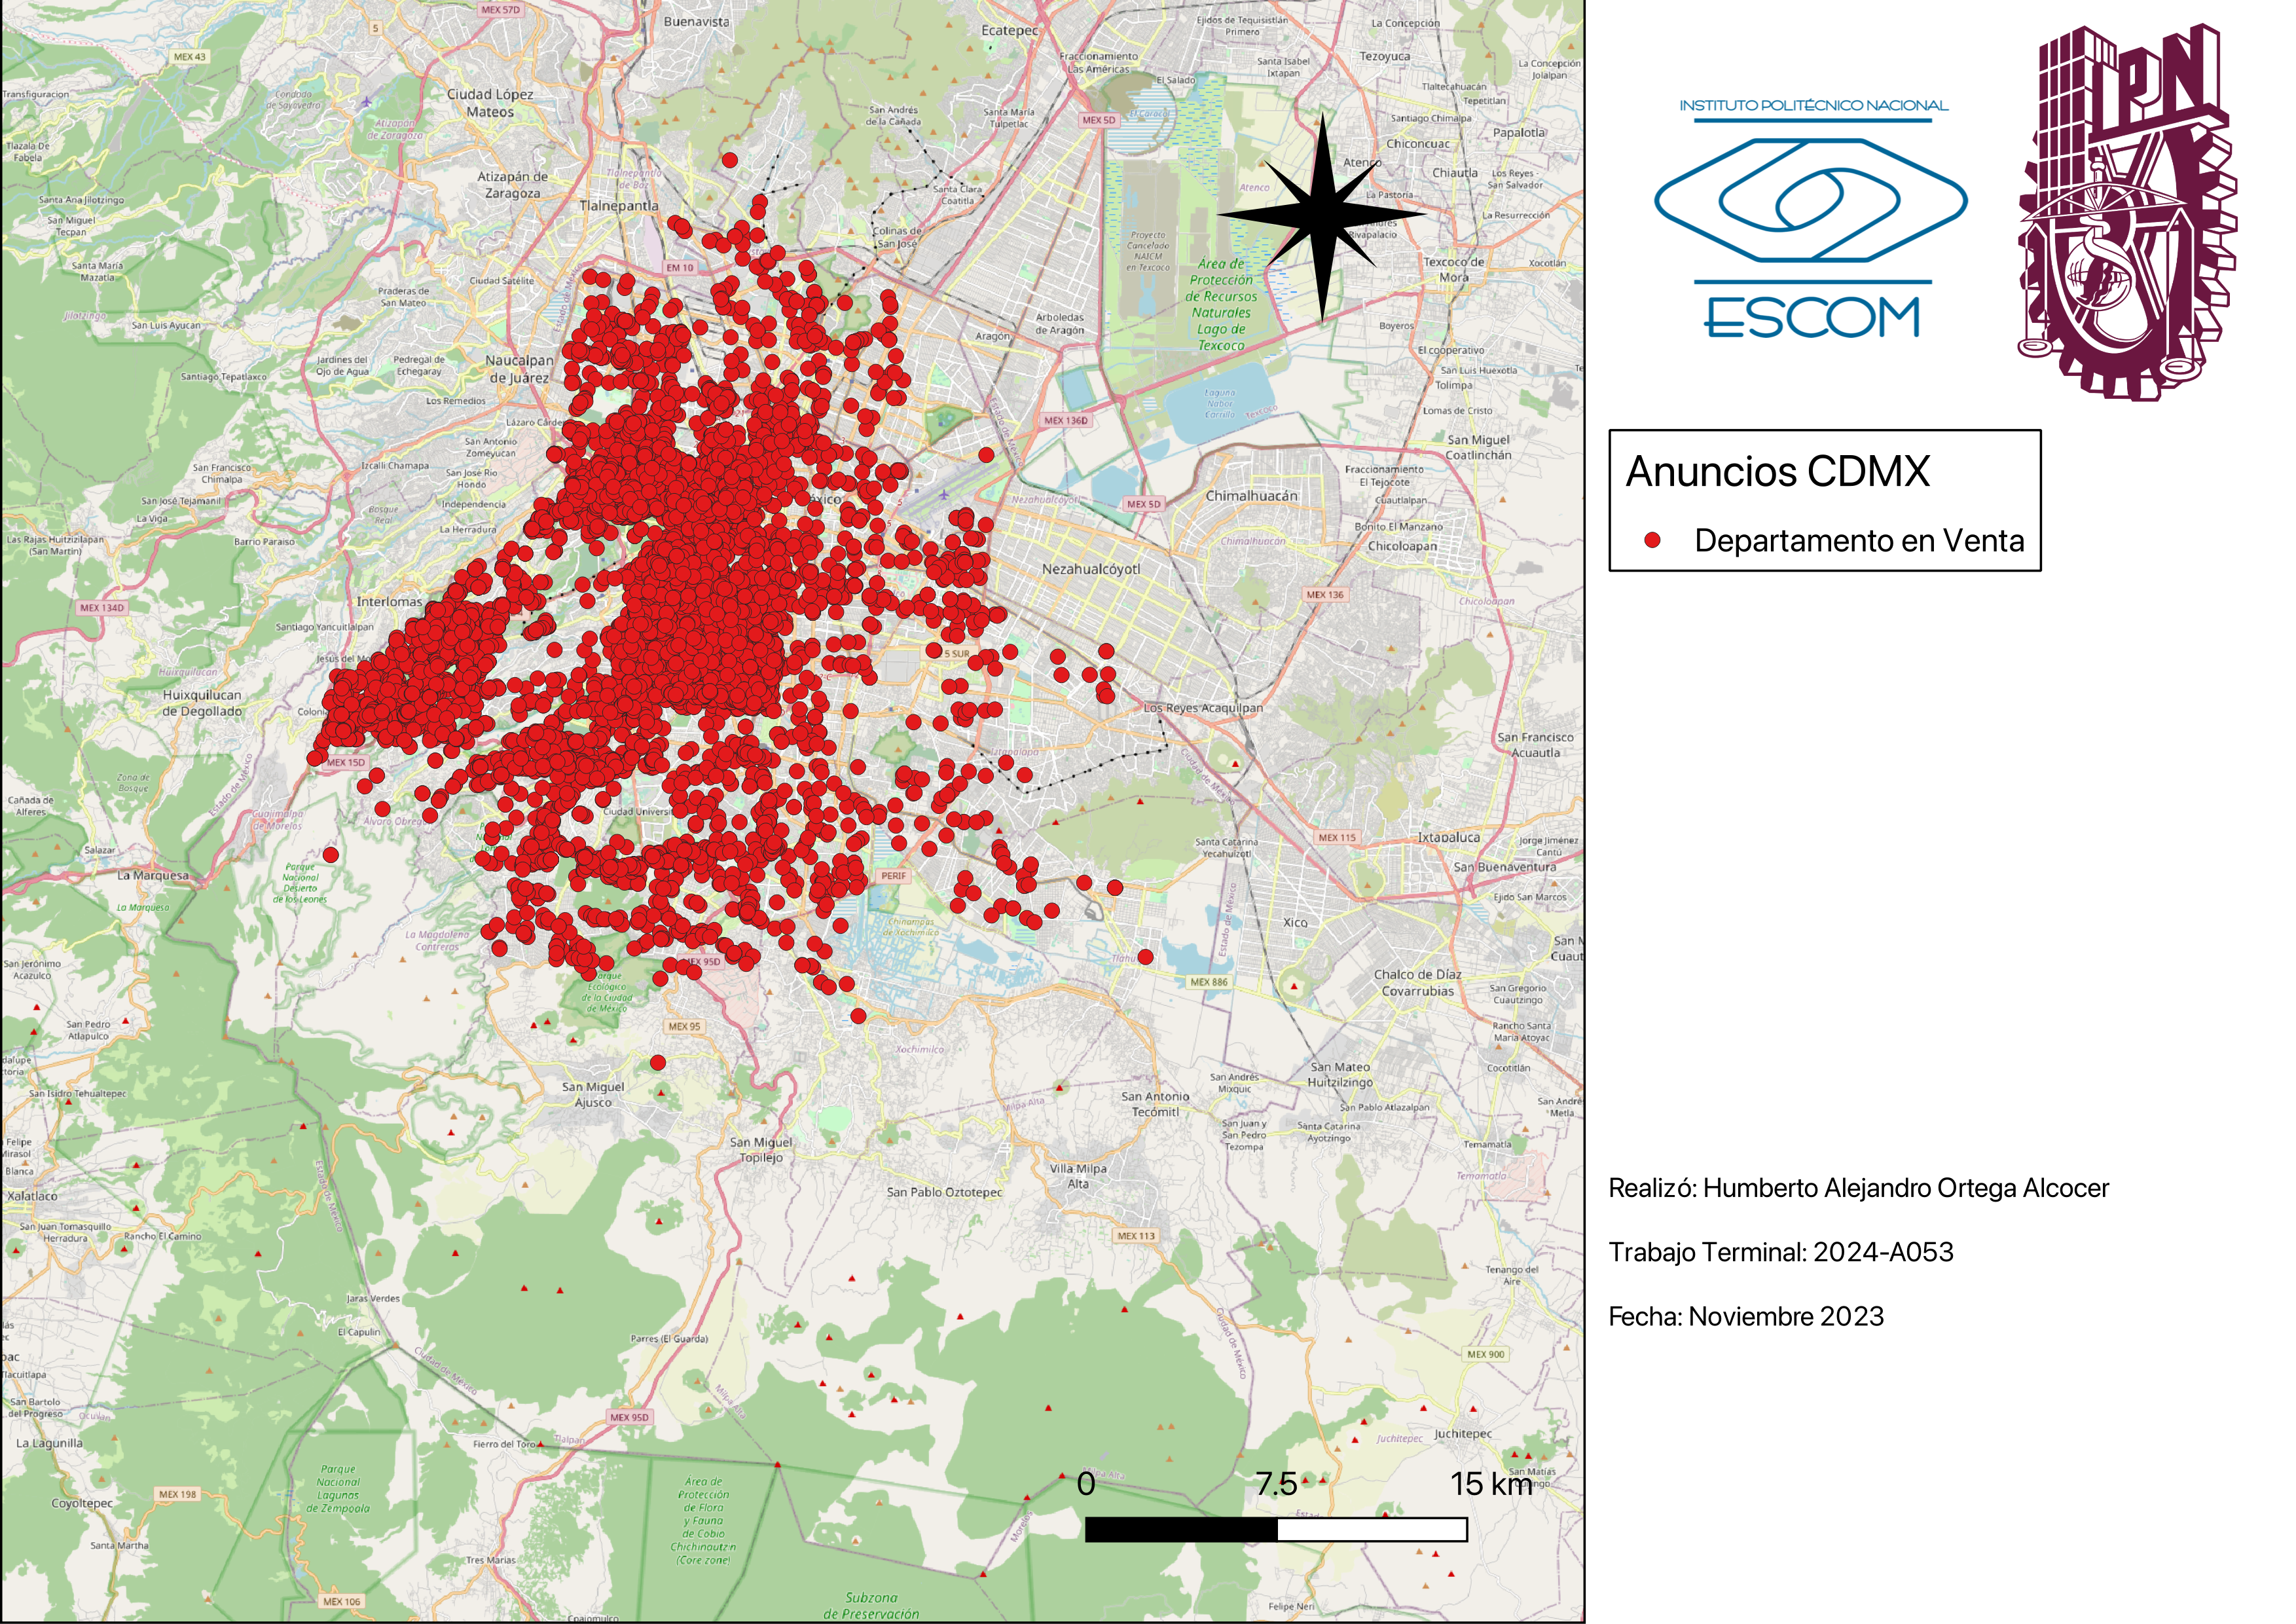
\includegraphics[width=0.8\textwidth]{imagenes/03-analisis/visualizacion-puntos-anuncios.png}
  \caption{Visualización de puntos de anuncios.}
  \label{fig:visualizacion_puntos_anuncios}
\end{figure}

De aquí, podemos derivar las siguientes conclusiones:

\begin{itemize}
  \item Los anuncios no se encuentran distribuidos de manera uniforme en toda la
  Ciudad de México.
  \item Los anuncios se encuentran distribuidos de manera uniforme en las
  alcaldías Cuauhtémoc, Benito Juárez y Miguel Hidalgo.
\item En las alcaldías Milpa Alta y Xochimilco existen pocos anuncios debido a
  que son zonas con poca densidad de población y muchos tratos aún se realizan
    de manera tradicional (sin el uso de plataformas online).
\end{itemize}

\subsubsection{Mapa de densidad de anuncios por alcaldía}

El mapa de densidad de anuncios permite visualizar la concentración de
anuncios en las diferentes alcaldías de la CDMX. Esto permite identificar las áreas con alta y baja
densidad de anuncios y posibles factores (desarrollo urbano, demanda, etc.). En
la Figura \ref{fig:mapa_calor_densidad_anuncios} se muestra el mapa de calor de
densidad de anuncios para el conjunto de datos de bienes raíces.

\begin{figure}[H]
  \centering
  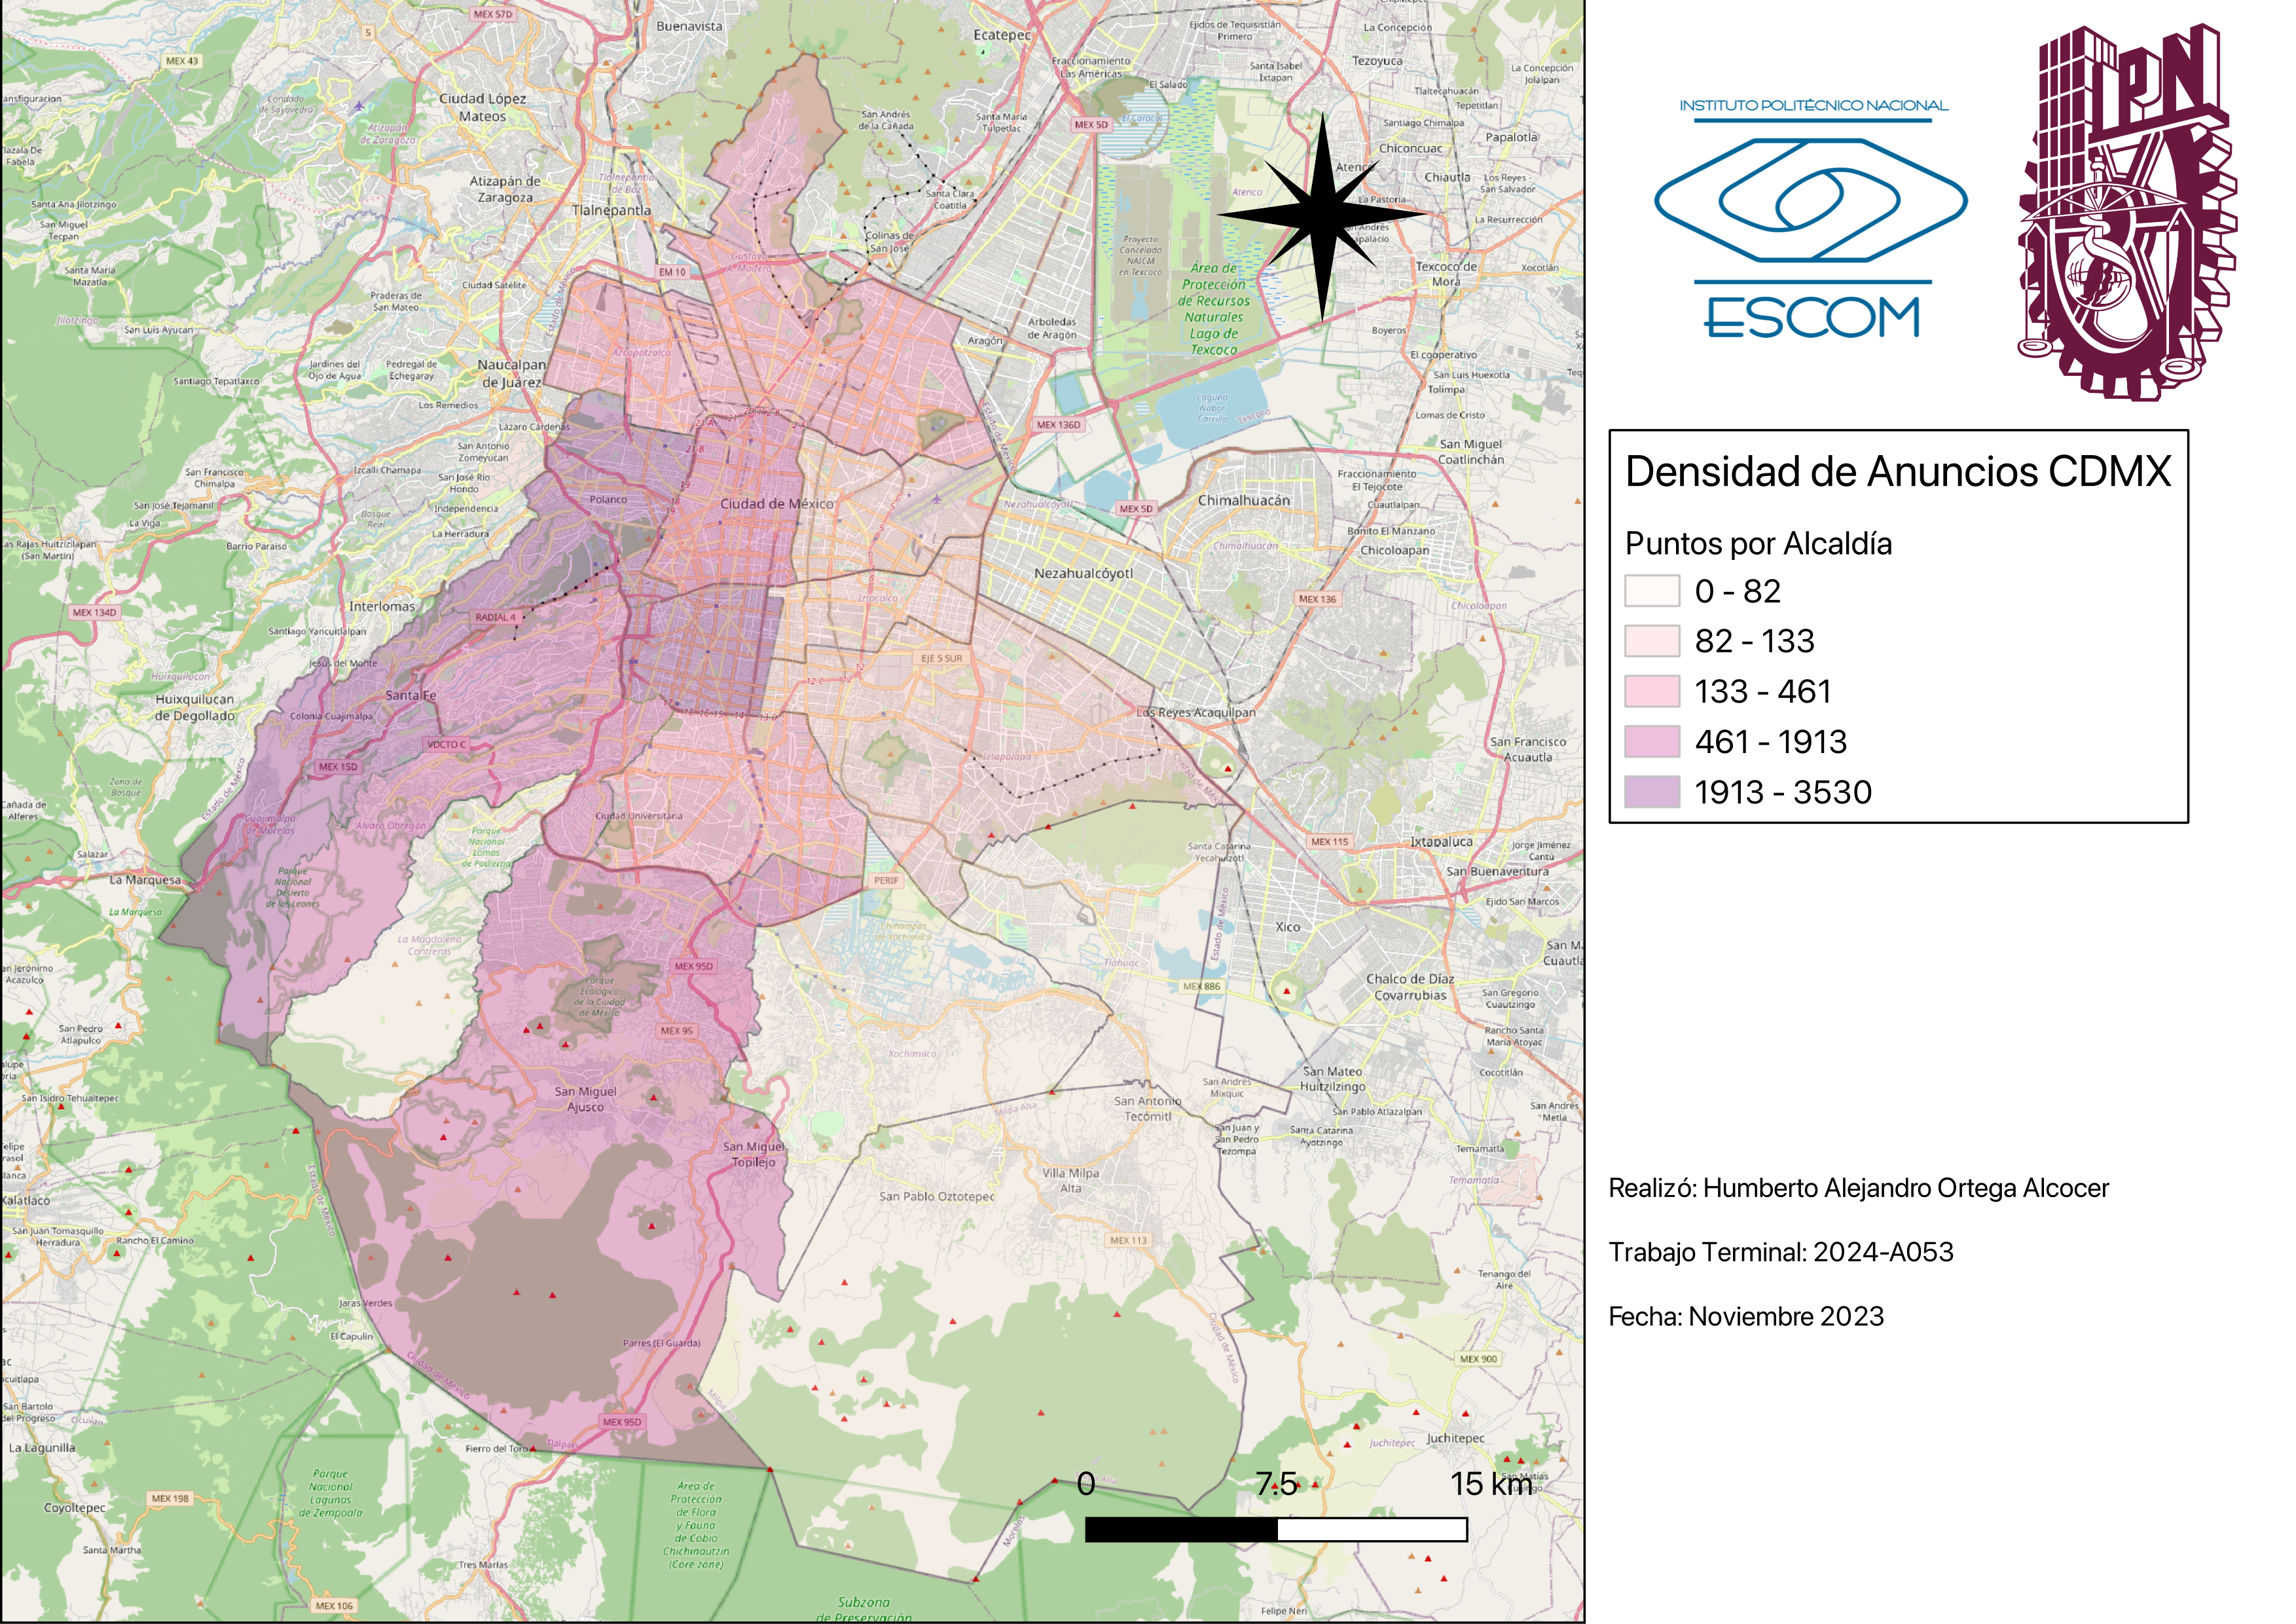
\includegraphics[width=0.8\textwidth]{imagenes/03-analisis/mapa-densidad-anuncios.png}
  \caption{Mapa de de densidad de anuncios por alcaldía.}
  \label{fig:mapa_calor_densidad_anuncios}
\end{figure}

De aquí, podemos derivar las siguientes conclusiones:

\begin{itemize}
  \item Las zonas con mayor densidad de anuncios se encuentran en la zona centro
  de la Ciudad de México, en las alcaldías Cuauhtémoc y Miguel Hidalgo.
  \item Las zonas con menor densidad de anuncios se encuentran en la zona sur
  de la Ciudad de México, en las alcaldías Tlalpan, Xochimilco y Milpa Alta.
\end{itemize}

Los datos correspondientes al mapa de la Figura \ref{fig:mapa_calor_densidad_anuncios}
se muestran en el Cuadro \ref{table:mapa_calor_densidad_anuncios}.

\begin{table}[H]
\centering
\begin{tabular}{|l|l|}
\hline
\rowcolor{azulclaro}
%\centering\textbf{Alcaldía} & \centering\textbf{Cantidad de Anuncios}\arraybackslash \\
\multicolumn{1}{|c|}{\textbf{Alcaldía}} & \multicolumn{1}{c|}{\textbf{Cantidad de Anuncios}} \\
\hline
Benito Juárez & 3530 \\
\hline
Miguel Hidalgo & 3114 \\
\hline
Cuajimalpa de Morelos & 2246 \\
\hline
Cuauhtémoc & 1913 \\
\hline
Álvaro Obregón & 1711 \\
\hline
Tlalpan & 483 \\
\hline
Coyoacán & 461 \\
\hline
Azcapotzalco & 301 \\
\hline
Gustavo A. Madero & 191 \\
\hline
Iztacalco & 133 \\
\hline
Venustiano Carranza & 127 \\
\hline
Iztapalapa & 117 \\
\hline
La Magdalena Contreras & 82 \\
\hline
Tláhuac & 29 \\
\hline
Xochimilco & 16 \\
\hline
Milpa Alta & 0 \\
\hline
\end{tabular}
\caption{Datos correspondientes al número de anuncios encontrados por alcaldía.}
\label{table:mapa_calor_densidad_anuncios}
\end{table}
\subsubsection{Mapa de calor de precios}

El mapa de calor de precios permite visualizar cómo se distribuyen los precios
en diferentes áreas. Esto permite identificar las zonas con precios más altos o
más bajos y posibles razones (ubicación, accesibilidad, etc.). En la Figura
\ref{fig:mapa_calor_precios} se muestra el mapa de calor de precios para el
conjunto de datos de bienes raíces.

\begin{figure}[H]
  \centering
  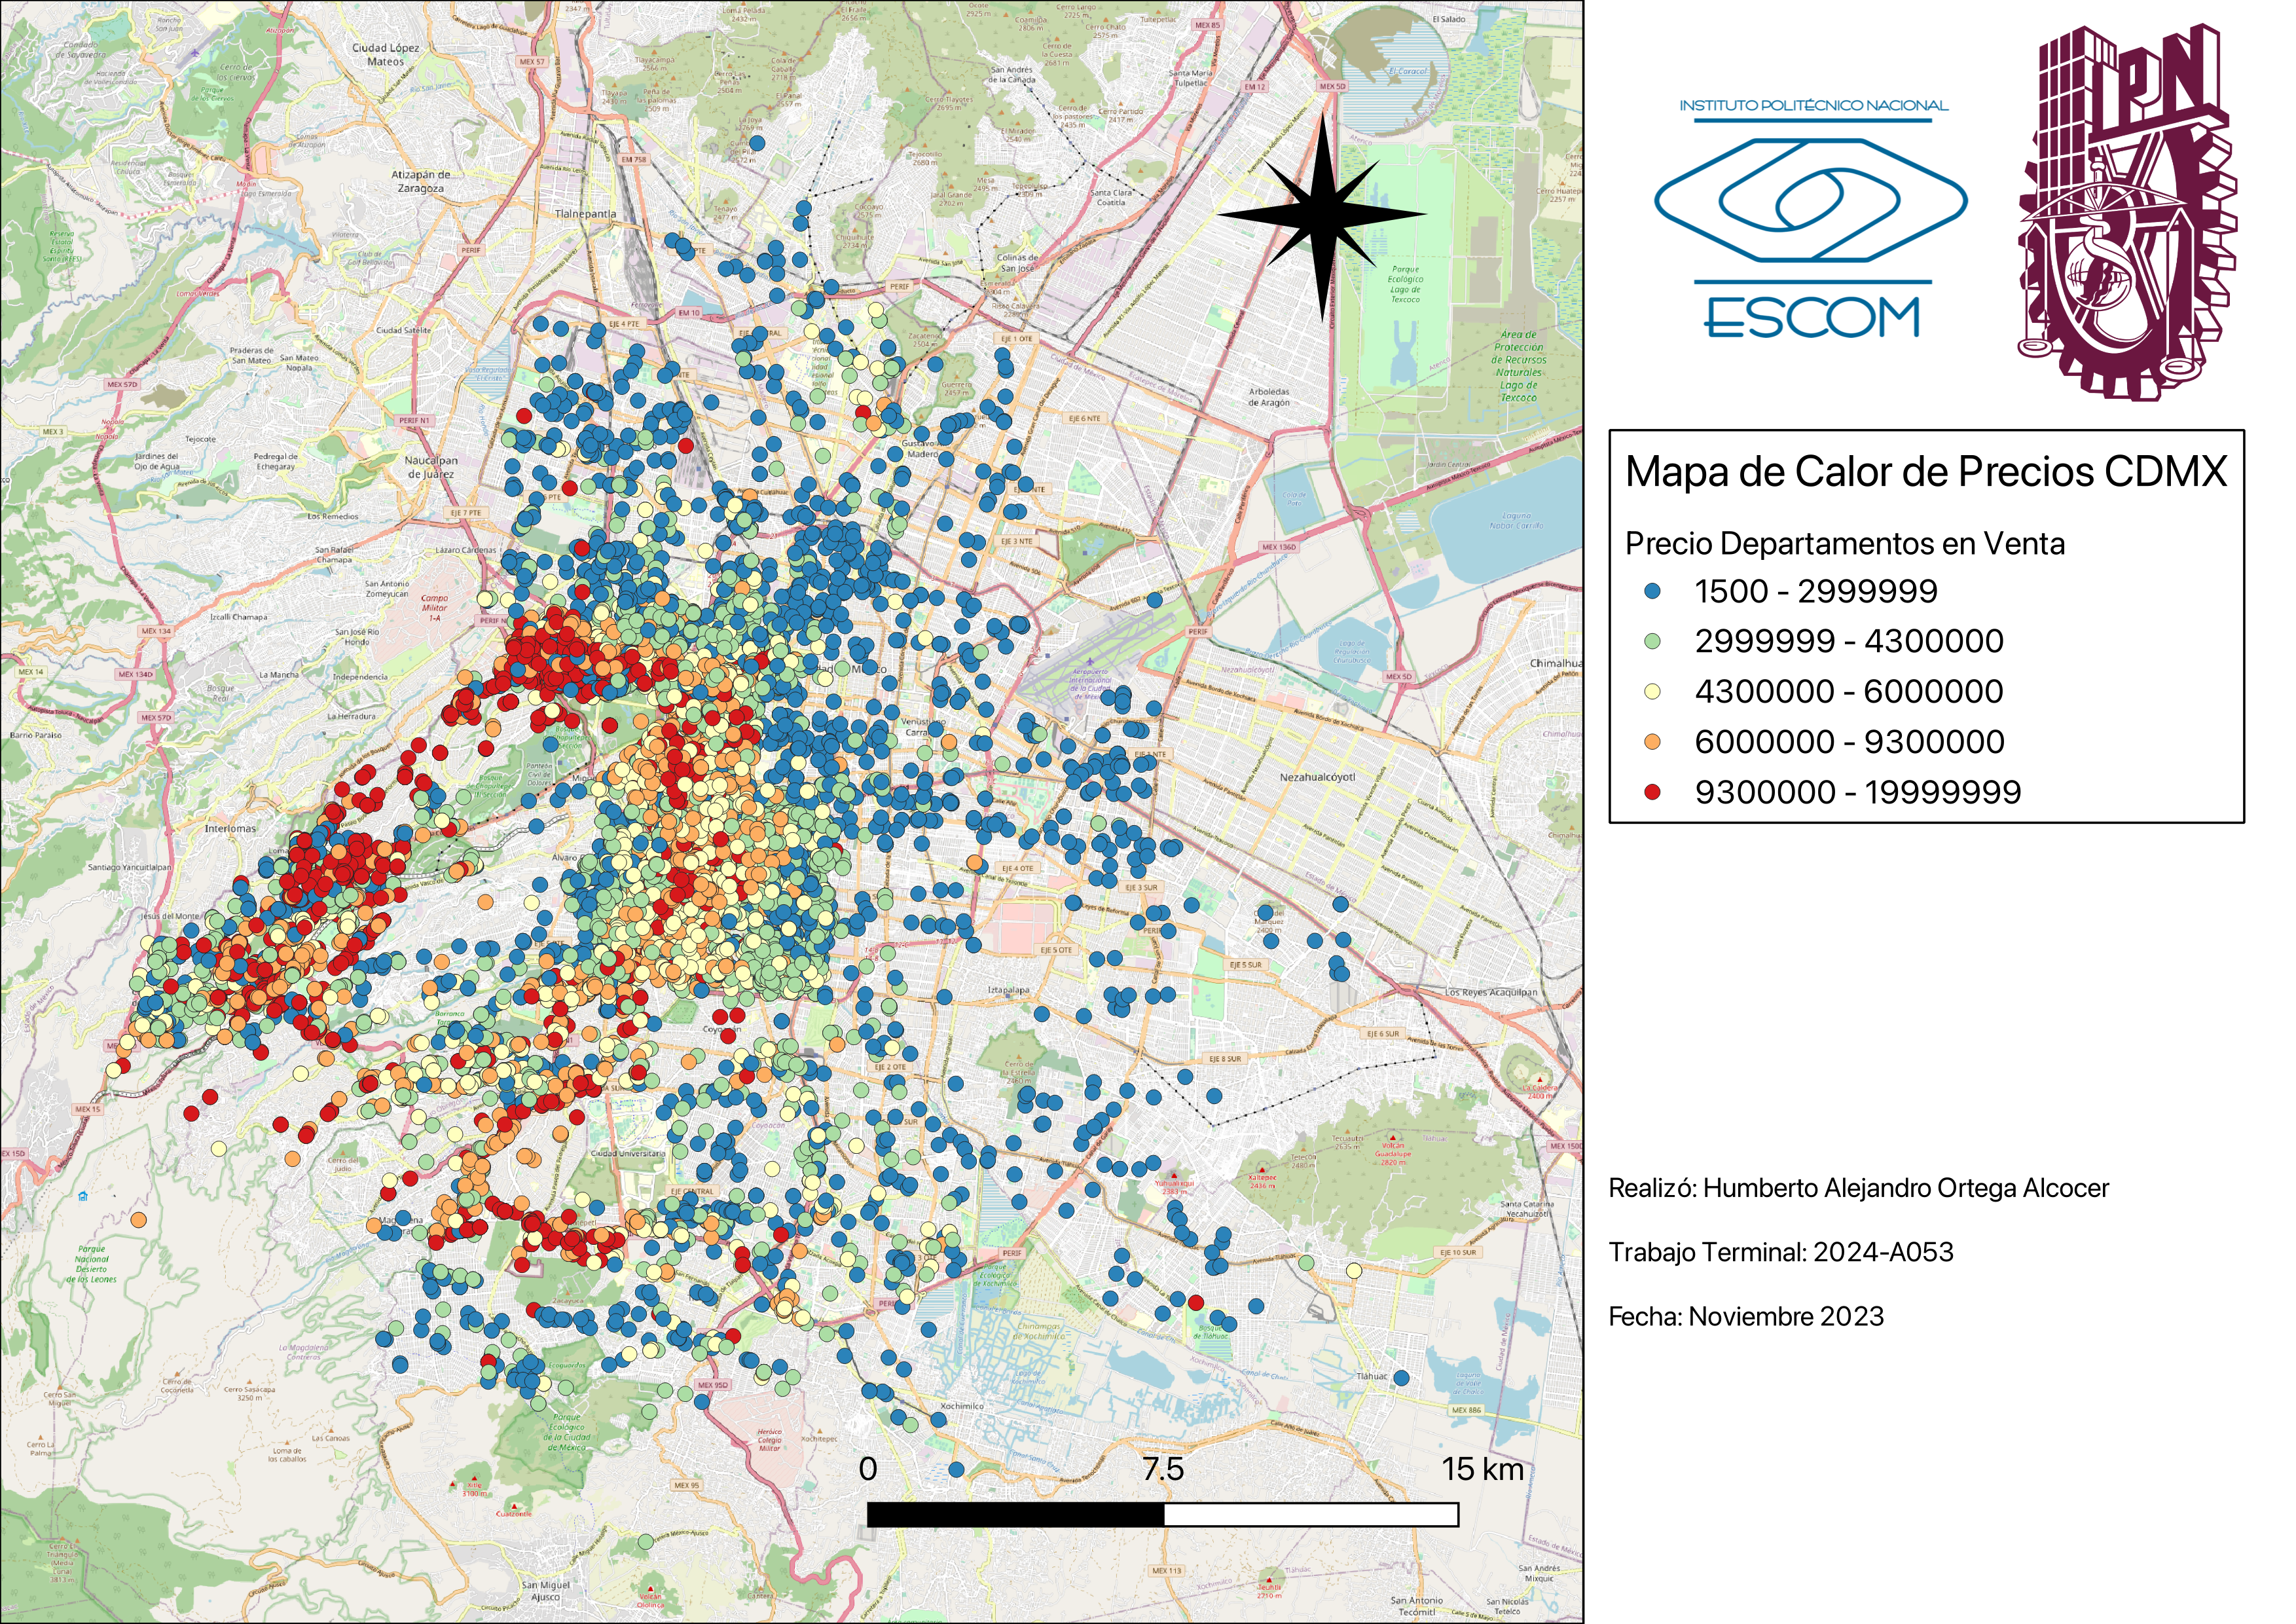
\includegraphics[width=0.9\textwidth]{imagenes/03-analisis/mapa-densidad-precio.png}
  \caption{Mapa de calor de precios.}
  \label{fig:mapa_calor_precios}
\end{figure}

De aquí, podemos derivar las siguientes conclusiones:

\begin{itemize}
  \item Los precios más altos se encuentran en la zona centro de la Ciudad de
  México, en las alcaldías Cuauhtémoc y Miguel Hidalgo.
  \item Los precios más bajos se encuentran en la zona sur de la Ciudad de
  México, en las alcaldías Tlalpan, Xochimilco y Milpa Alta.
\item Los precios más altos se encuentran en las zonas con mayor densidad de
  vegetación, como el Bosque de Chapultepec, el Parque Ecológico de Xochimilco
  y el Parque Ecológico de la Ciudad de México.
\end{itemize}

\subsubsection{Mapa de calor de número de recámaras}

El mapa de calor de número de recámaras permite visualizar cómo se distribuyen
los anuncios según el número de recámaras. Esto permite identificar las zonas
con mayor y menor número de recámaras y analizar si el precio es un factor
determinante en el número de recámaras. En la Figura \ref{fig:mapa_calor_recamaras}
se muestra el mapa de calor de número de recámaras para el conjunto de datos de
bienes raíces.

\begin{figure}[H]
  \centering
  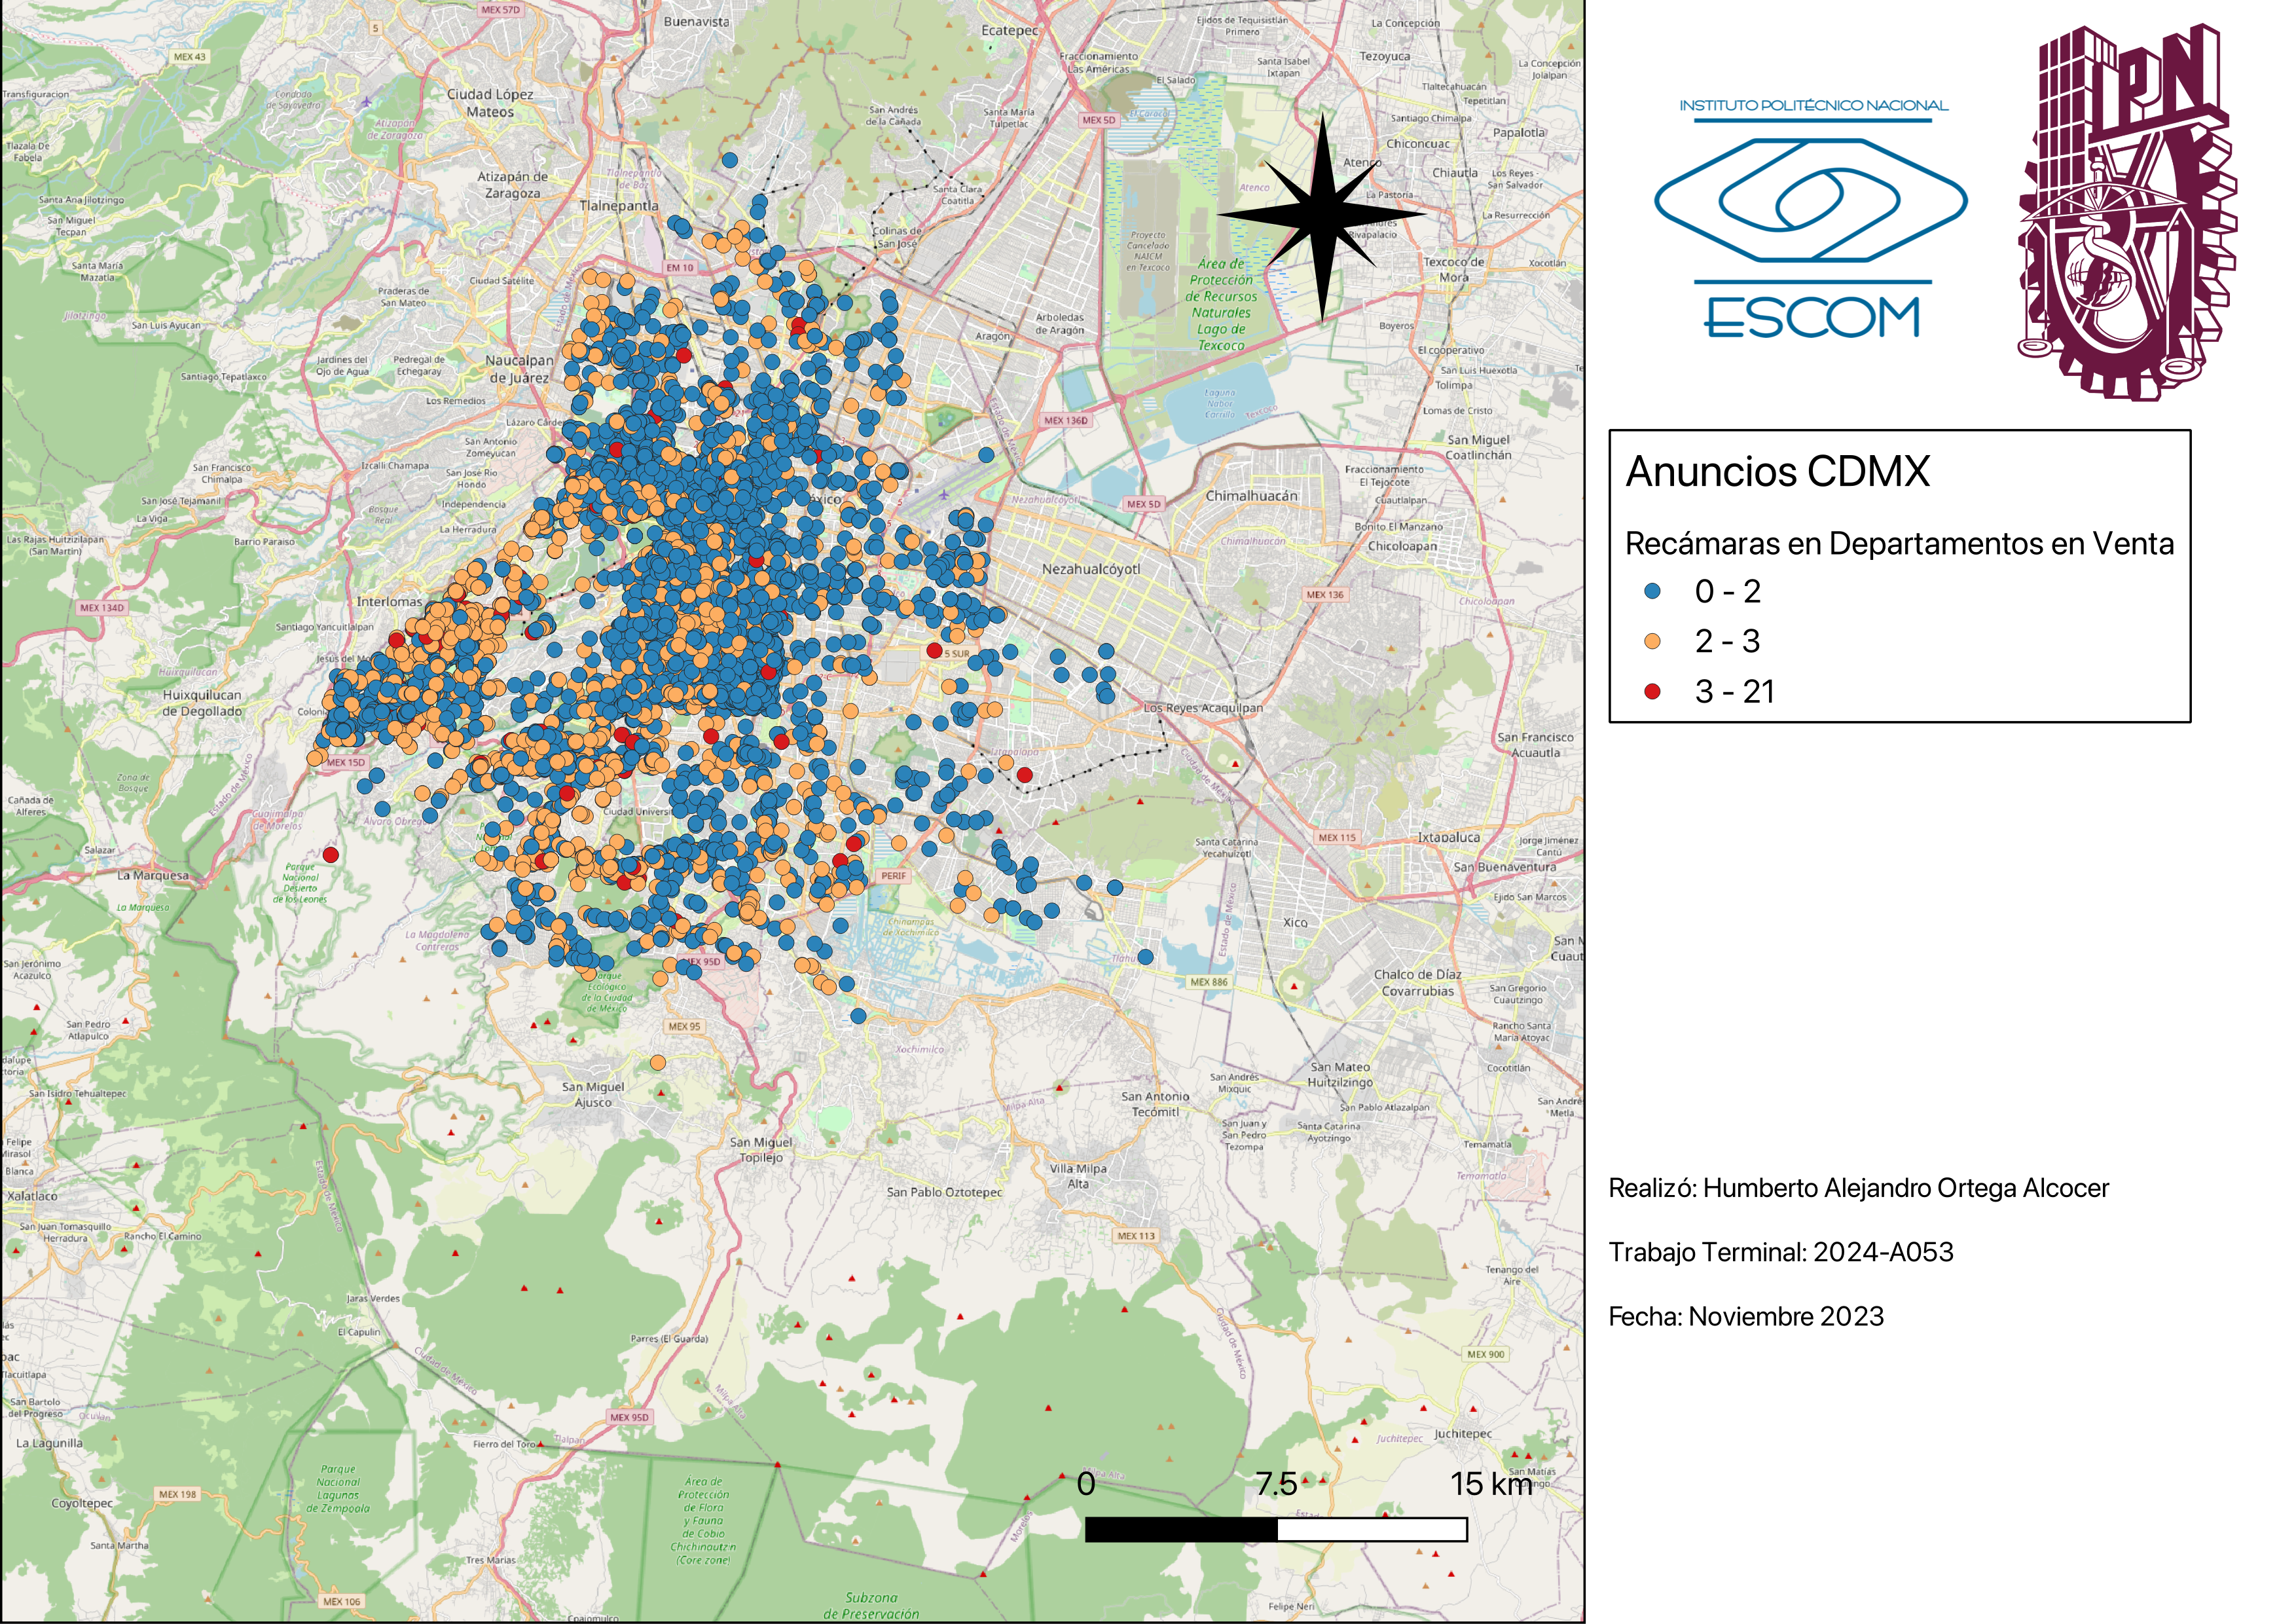
\includegraphics[width=0.9\textwidth]{imagenes/03-analisis/mapa-densidad-recamaras.png}
  \caption{Mapa de calor de número de recámaras.}
  \label{fig:mapa_calor_recamaras}
\end{figure}

De aquí, podemos derivar las siguientes conclusiones:

\begin{itemize}
  \item La gran mayoría de los departamentos en la Ciudad de México tienen 2 o
  3 recámaras.
  \item Los departamentos con 1 recámara se encuentran en las zonas con mayor
  densidad de población, como la zona centro de la Ciudad de México.
  \item Los departamentos con 4 o más recámaras se encuentran en las zonas con
  mayor precio, como la zona poniene de la Ciudad de México.
\end{itemize}

\subsubsection{Mapa de calor de número de baños}

Los baños nos indican la disponibilidad de servicios sanitarios en el inmueble,
así como un aproximado del número de personas que podrían habitar el mismo. En
la Figura \ref{fig:mapa_calor_banos} se muestra el mapa de calor de número de
baños para el conjunto de datos de bienes raíces.

\begin{figure}[H]
  \centering
  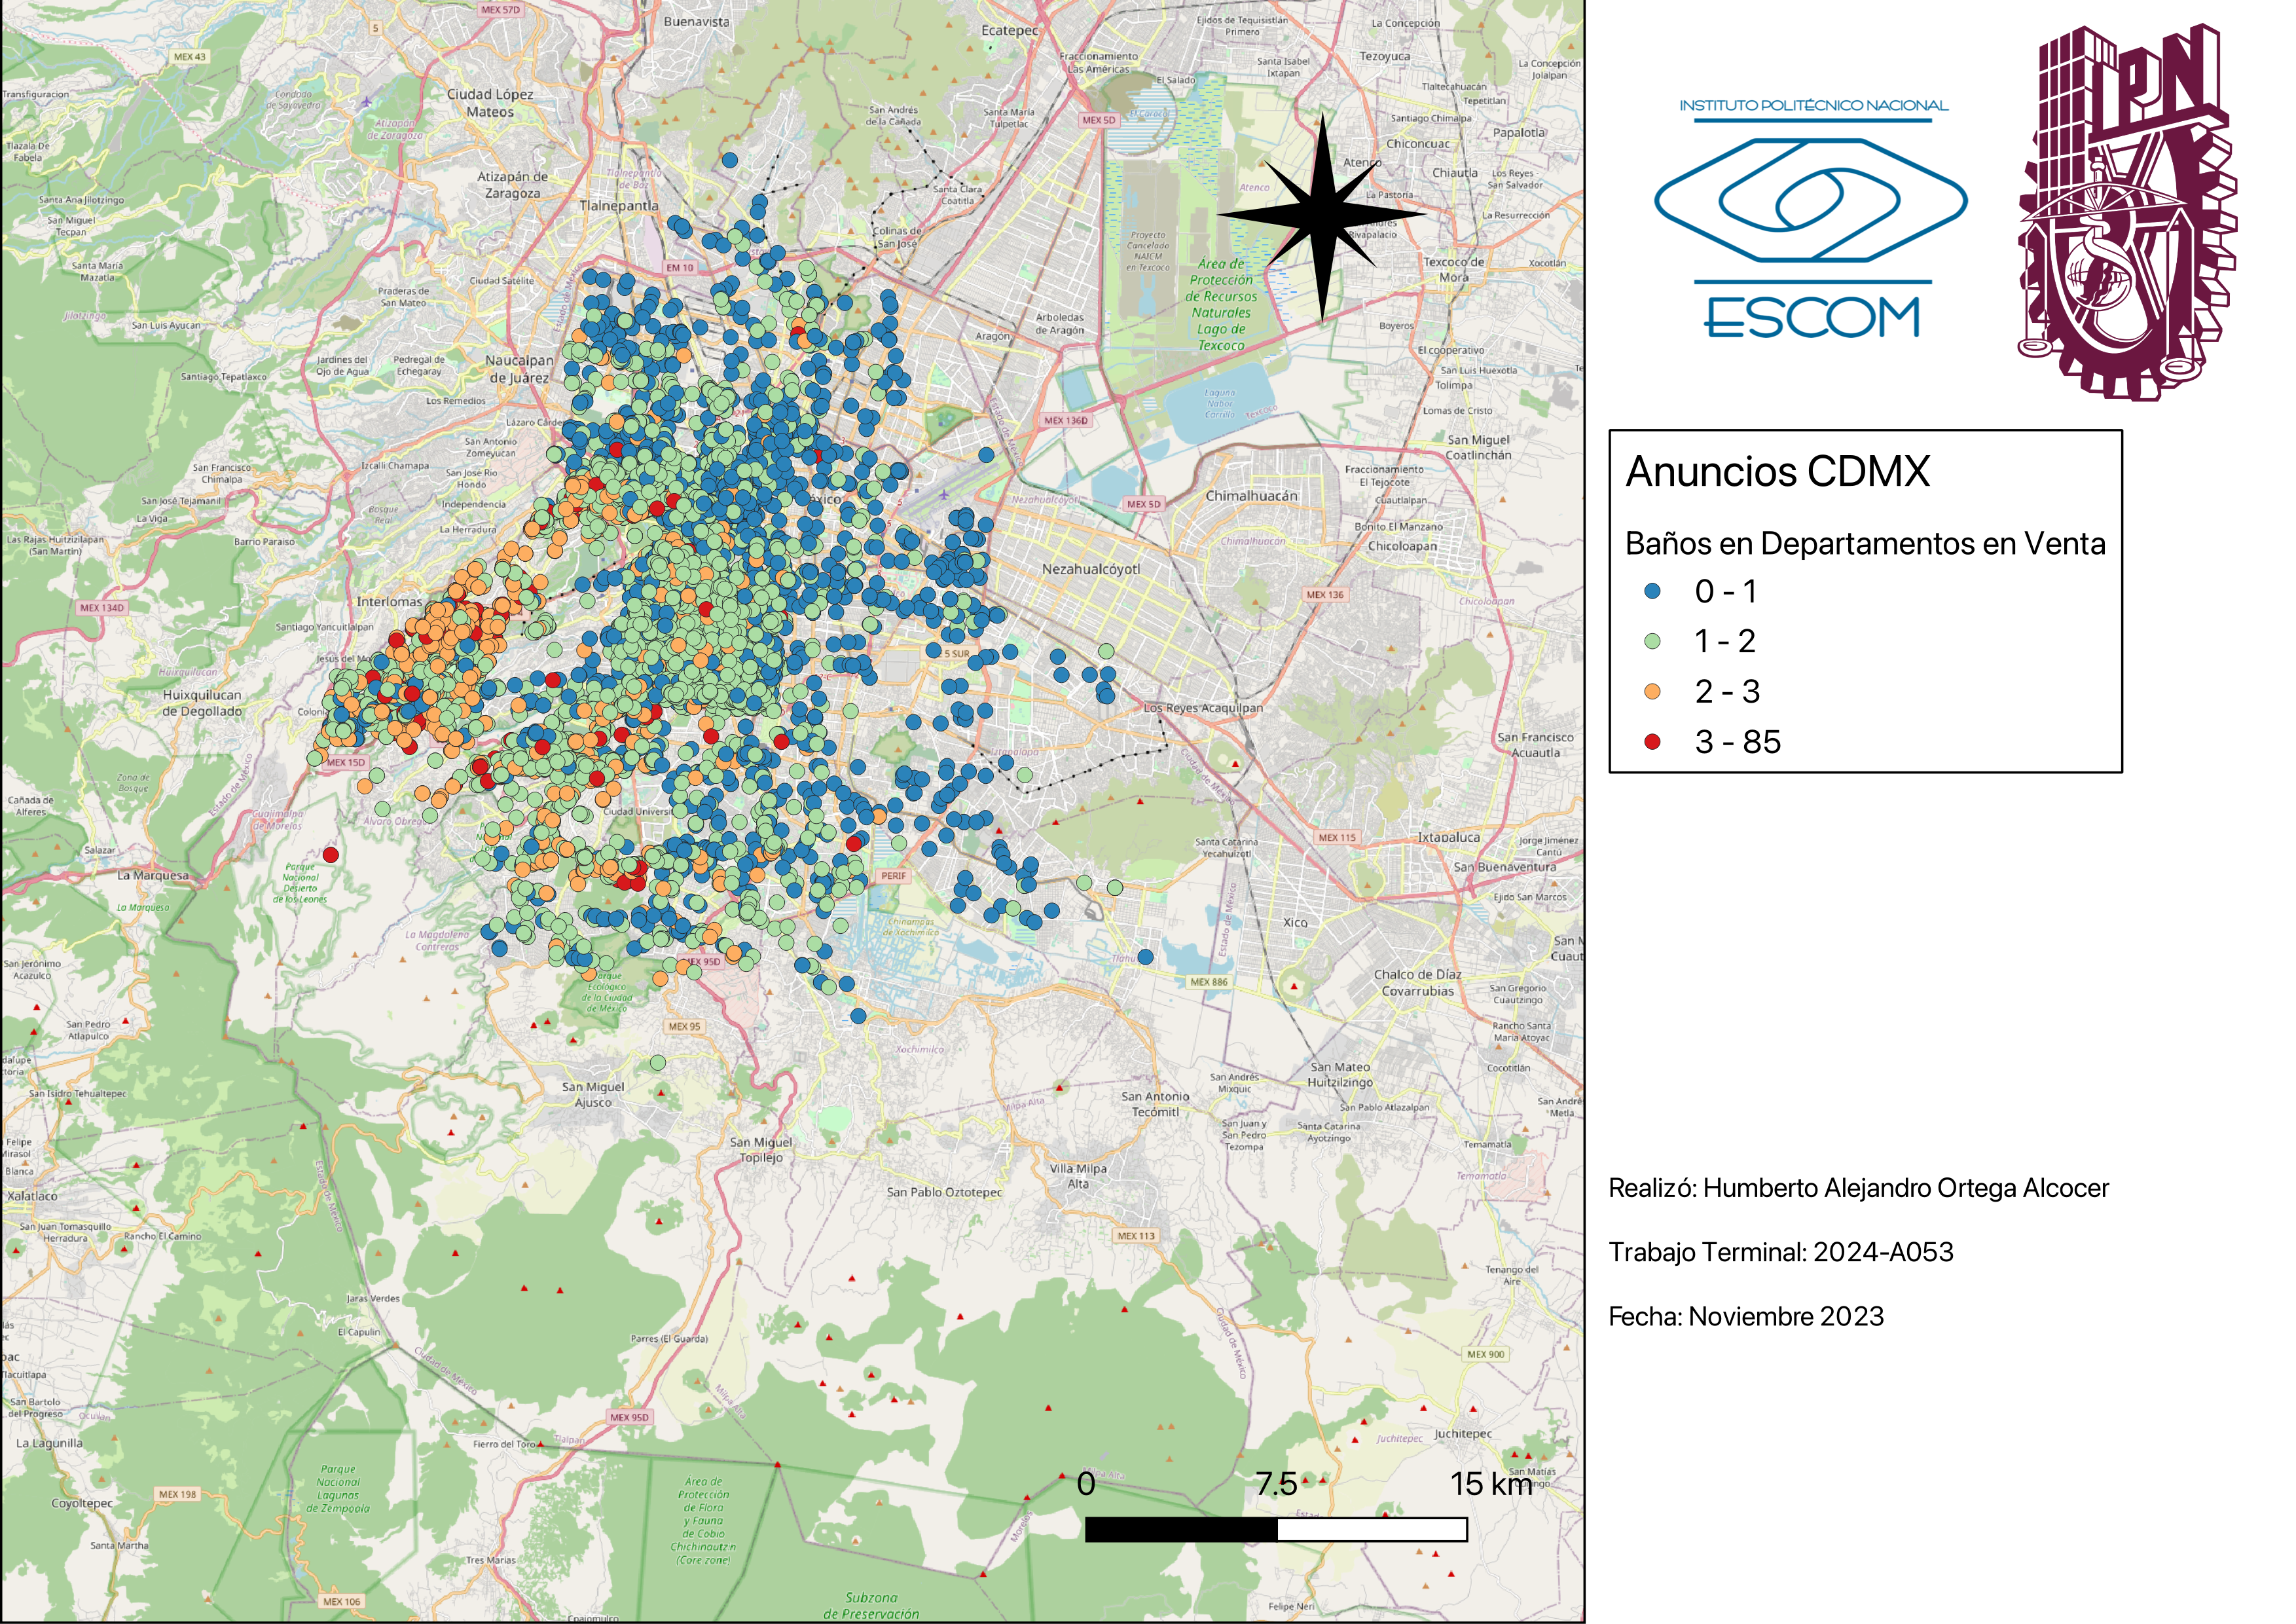
\includegraphics[width=0.9\textwidth]{imagenes/03-analisis/mapa-densidad-banos.png}
  \caption{Mapa de calor de número de baños.}
  \label{fig:mapa_calor_banos}
\end{figure}

De aquí, podemos derivar las siguientes conclusiones:

\begin{itemize}
  \item La gran mayoría de los departamentos en la Ciudad de México tienen 1 o
  2 baños.
  \item Los departamentos con 1 baño se encuentran en las zonas con mayor
  densidad de población, como la zona centro de la Ciudad de México.
  \item Los departamentos con 3 o más baños se encuentran en las zonas con
  mayor precio, como la zona poniene de la Ciudad de México.
\end{itemize}

\subsubsection{Mapa de calor de metros cuadrados}

La distribución de las superficies de departamentos en la Ciudad de México nos
permiten obtener un vistazo sobre la relación directa en el precio estimado
por metro cuadrado por zona, un factor determinante en el mercado inmobiliario.
En la Figura \ref{fig:mapa_calor_metros_cuadrados} se muestra el mapa de calor
de metros cuadrados para el conjunto de datos de bienes raíces.

\begin{figure}[H]
  \centering
  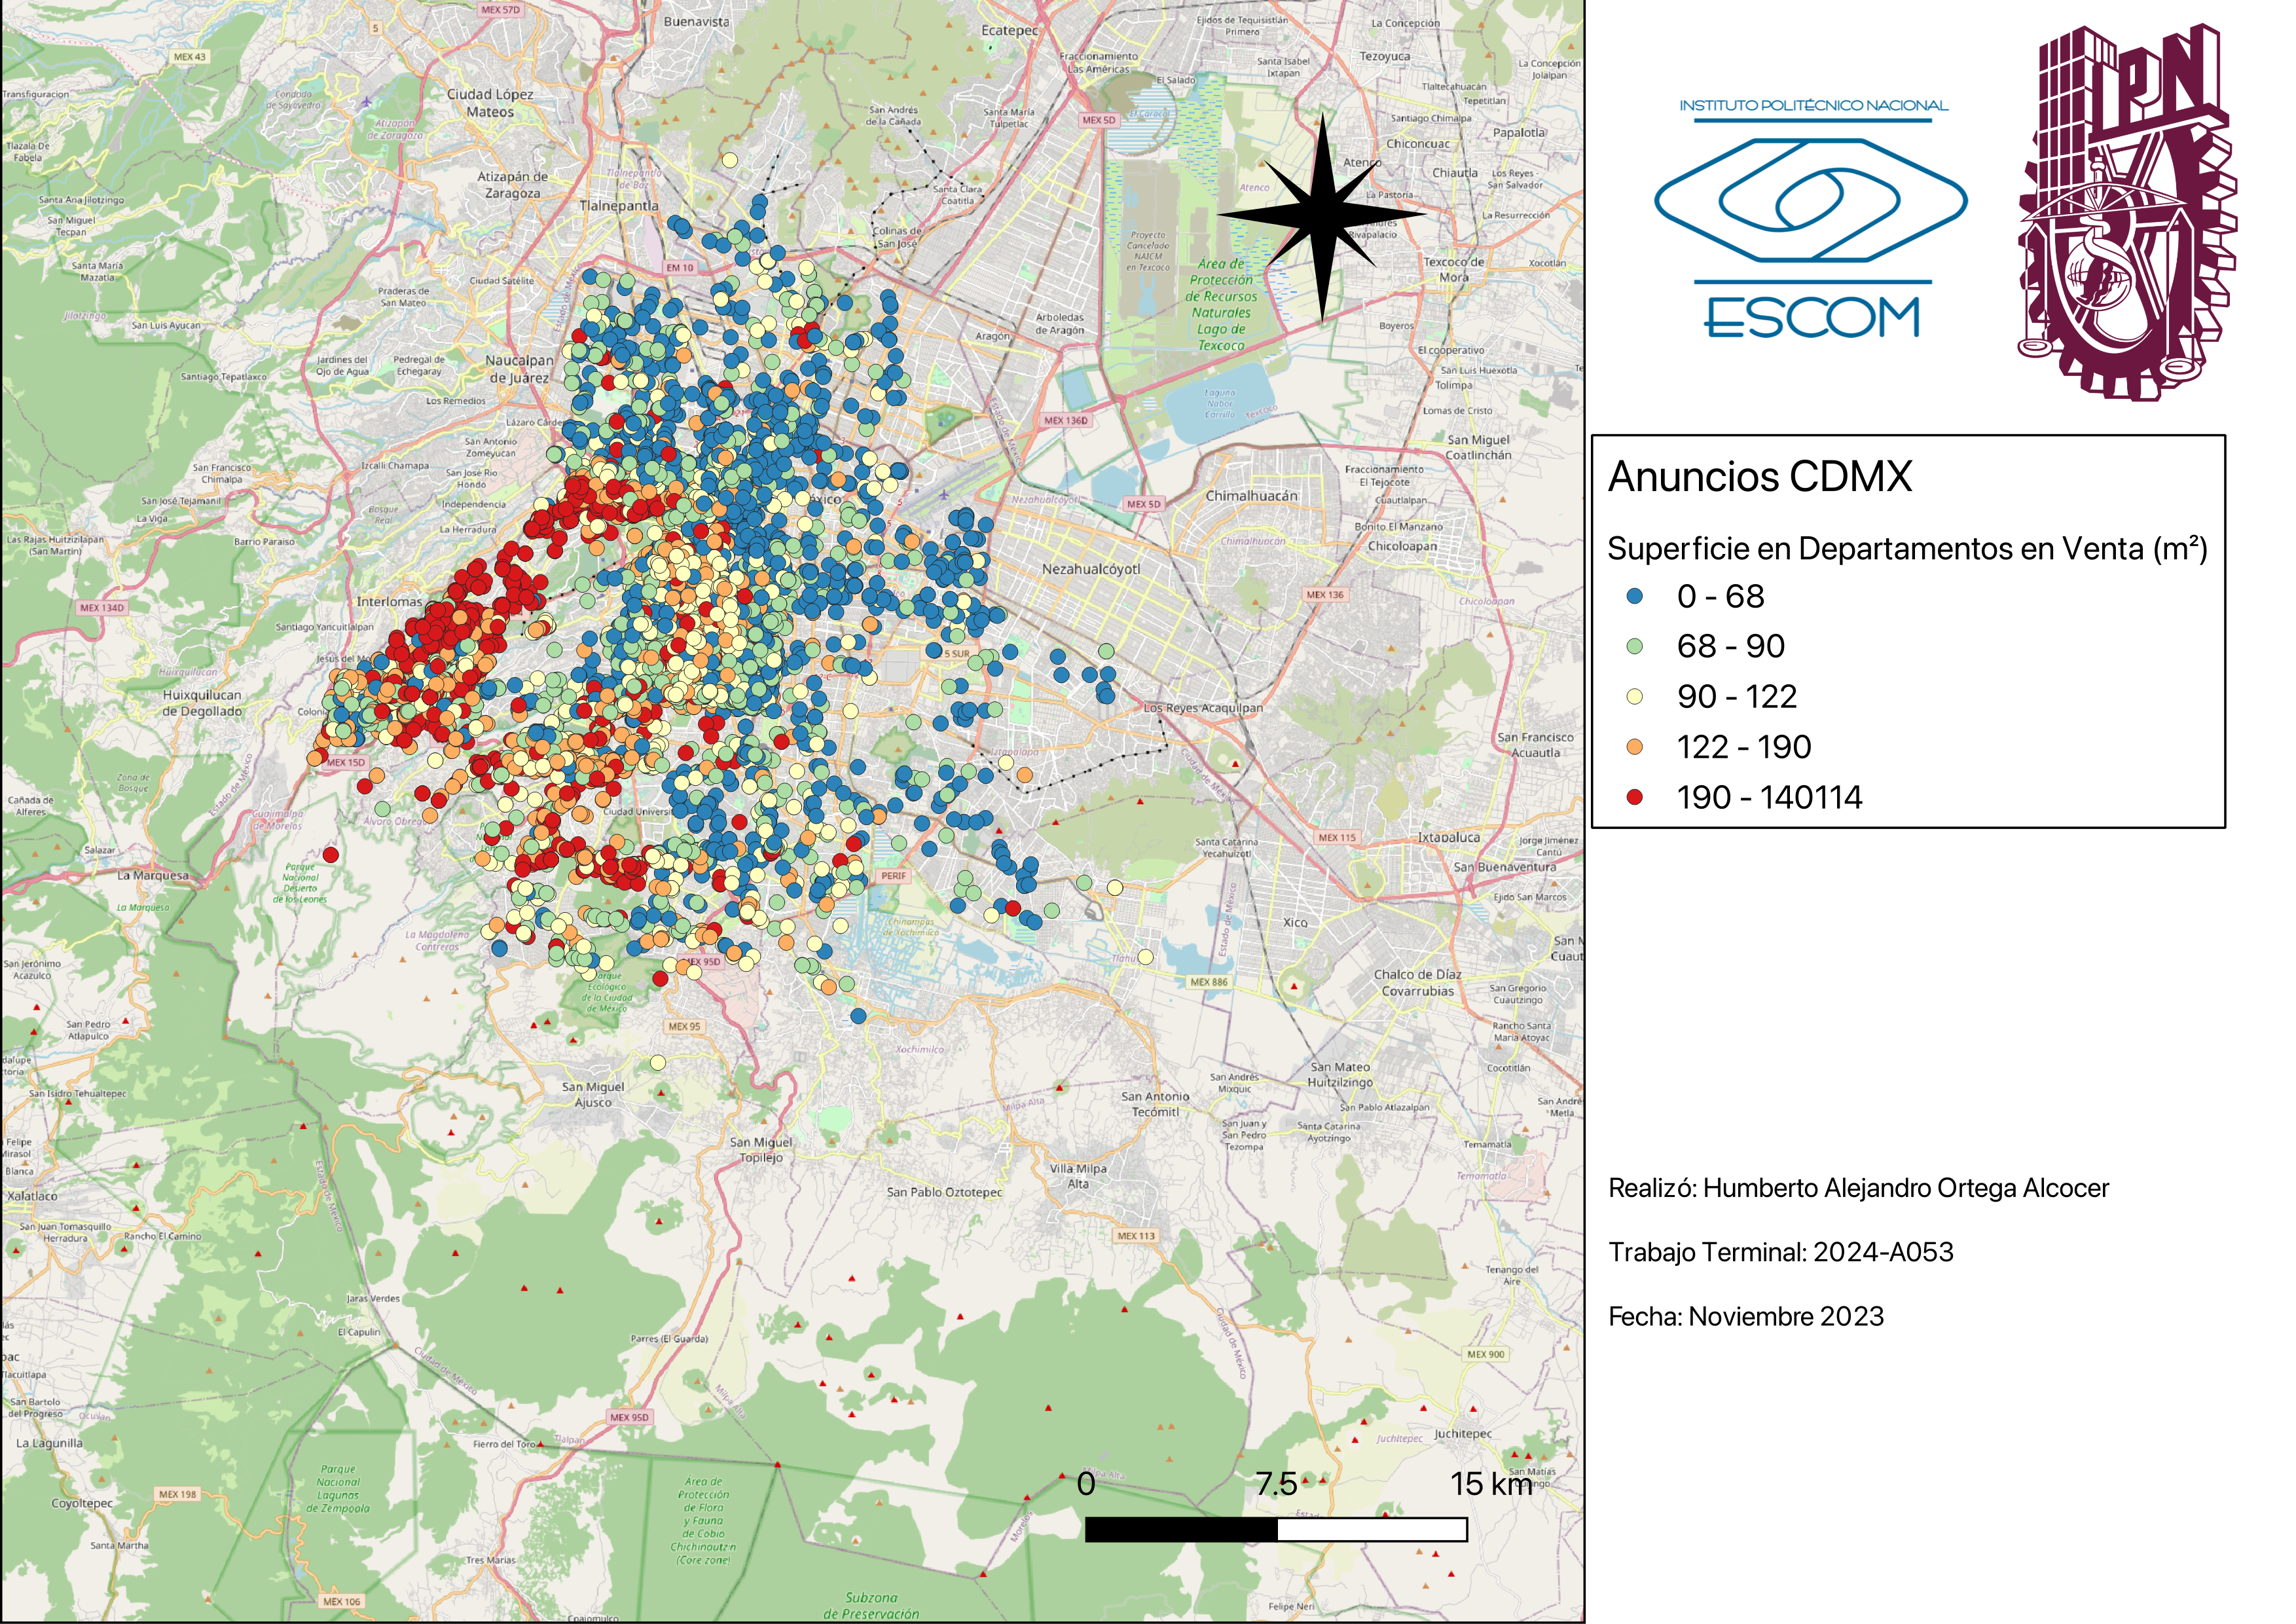
\includegraphics[width=0.9\textwidth]{imagenes/03-analisis/mapa-densidad-metros-cuadrados.png}
  \caption{Mapa de calor de metros cuadrados.}
  \label{fig:mapa_calor_metros_cuadrados}
\end{figure}

De aquí, podemos derivar las siguientes conclusiones:

\begin{itemize}
  \item La gran mayoría de los departamentos en la Ciudad de México tienen entre
  50 y 100 metros cuadrados.
  \item Los departamentos con menos de 50 metros cuadrados se encuentran en las
  zonas con mayor densidad de población, como la zona centro de la Ciudad de
  México. A su vez, estos departamentos tienen un precio por metro cuadrado más
  alto.
  \item Los departamentos con más de 100 metros cuadrados se encuentran en las
  zonas con mayor precio, como la zona poniene de la Ciudad de México.
\end{itemize}

\subsubsection{Mapa de calor de antigüedad}

La antigüedad de los departamentos es un factor determinante en el precio de los
mismos, ya que los departamentos más antiguos tienden a tener un precio más bajo
que los departamentos nuevos. Por otra parte, aunque no es el único factor a
considerar, al ser una zona sísmica, la antigüedad de los departamentos es un
factor importante a considerar para la seguridad de los habitantes. En la Figura
\ref{fig:mapa_calor_antiguedad} se muestra el mapa de calor de antigüedad para
el conjunto de datos de bienes raíces.

\begin{figure}[H]
  \centering
  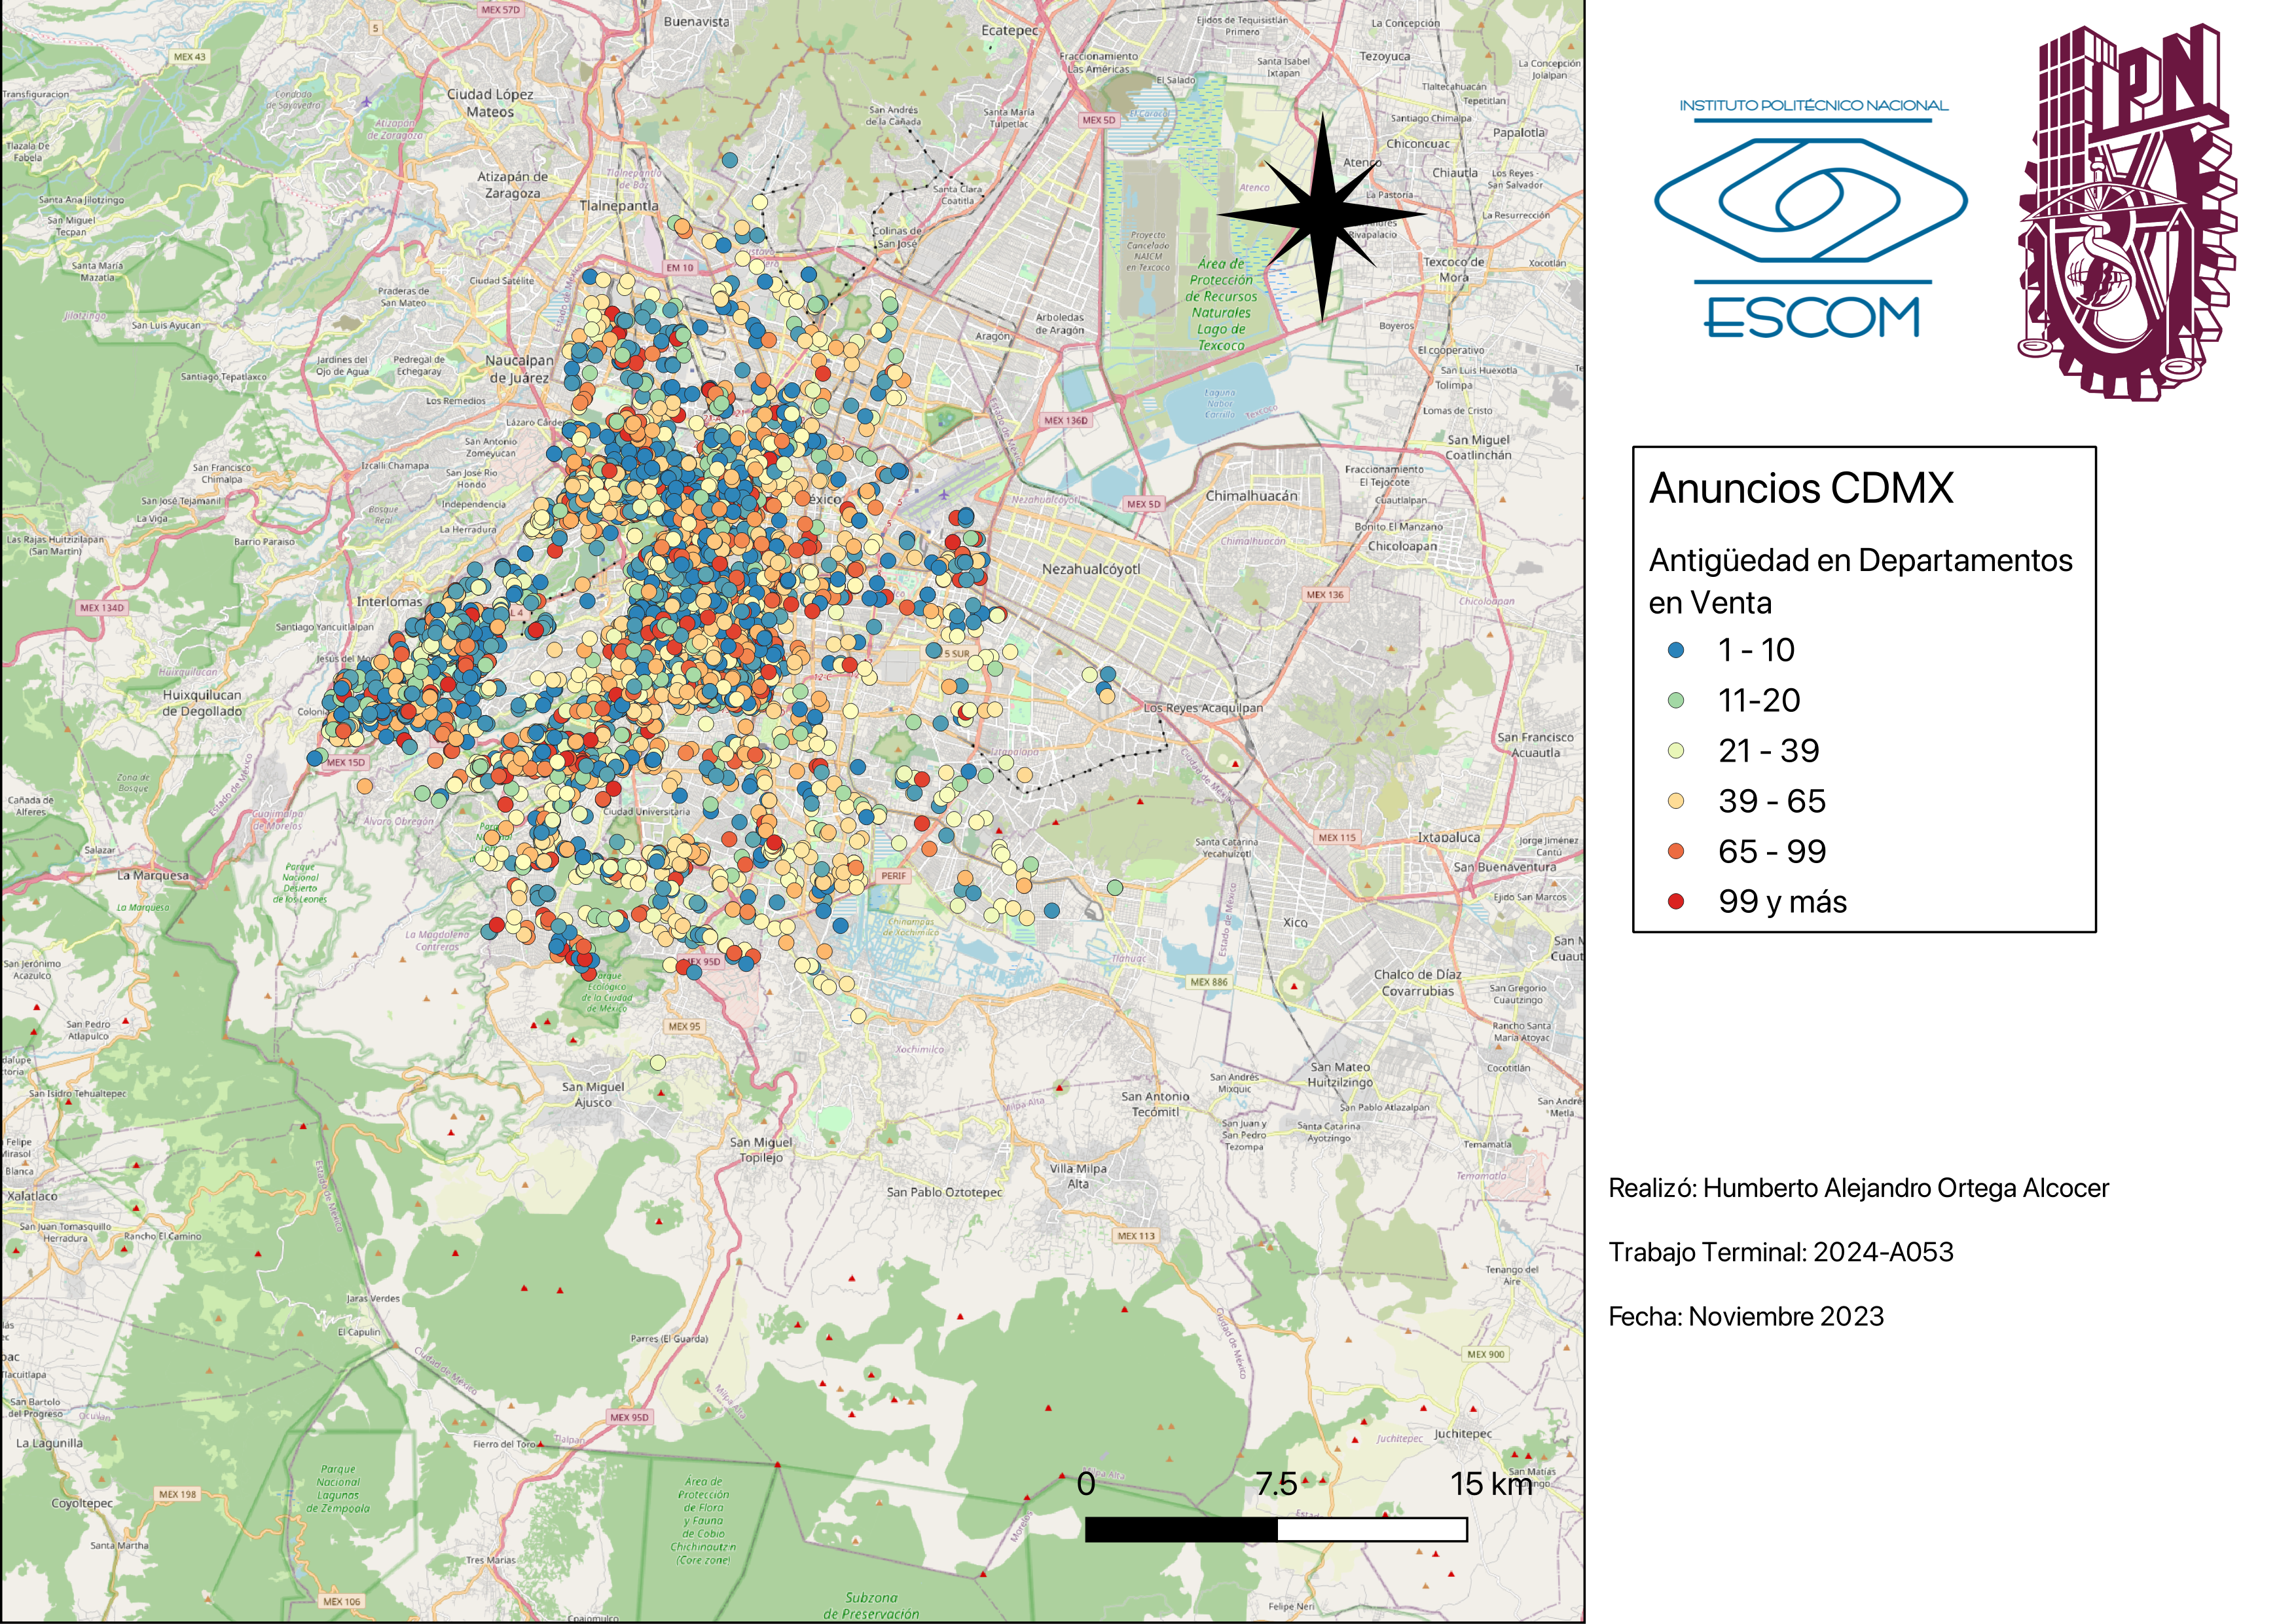
\includegraphics[width=0.9\textwidth]{imagenes/03-analisis/mapa-densidad-antiguedad.png}
  \caption{Mapa de calor de antigüedad.}
  \label{fig:mapa_calor_antiguedad}
\end{figure}

De aquí, podemos derivar las siguientes conclusiones:

\begin{itemize}
  \item La gran mayoría de los departamentos en la Ciudad de México tienen entre
  0 y 20 años de antigüedad.
  \item Los departamentos con menos de 20 años de antigüedad se encuentran en las
  zonas con mayor densidad de población, como la zona centro de la Ciudad de
  México. A su vez, estos departamentos tienen un precio más alto.
  \item Los departamentos con más de 20 años de antigüedad se encuentran en las
  zonas con mayor precio, como la zona poniene de la Ciudad de México.
\end{itemize}

\subsubsection{Mapa de calor por número de estacionamientos}

Los estacionamientos son un factor muy importante en la Ciudad de México, ya que
una gran cantidad de personas utilizan automóvil para transportarse. En la
Figura \ref{fig:mapa_calor_estacionamientos} se muestra el mapa de calor de
número de estacionamientos para el conjunto de datos de bienes raíces.

\begin{figure}[H]
  \centering
  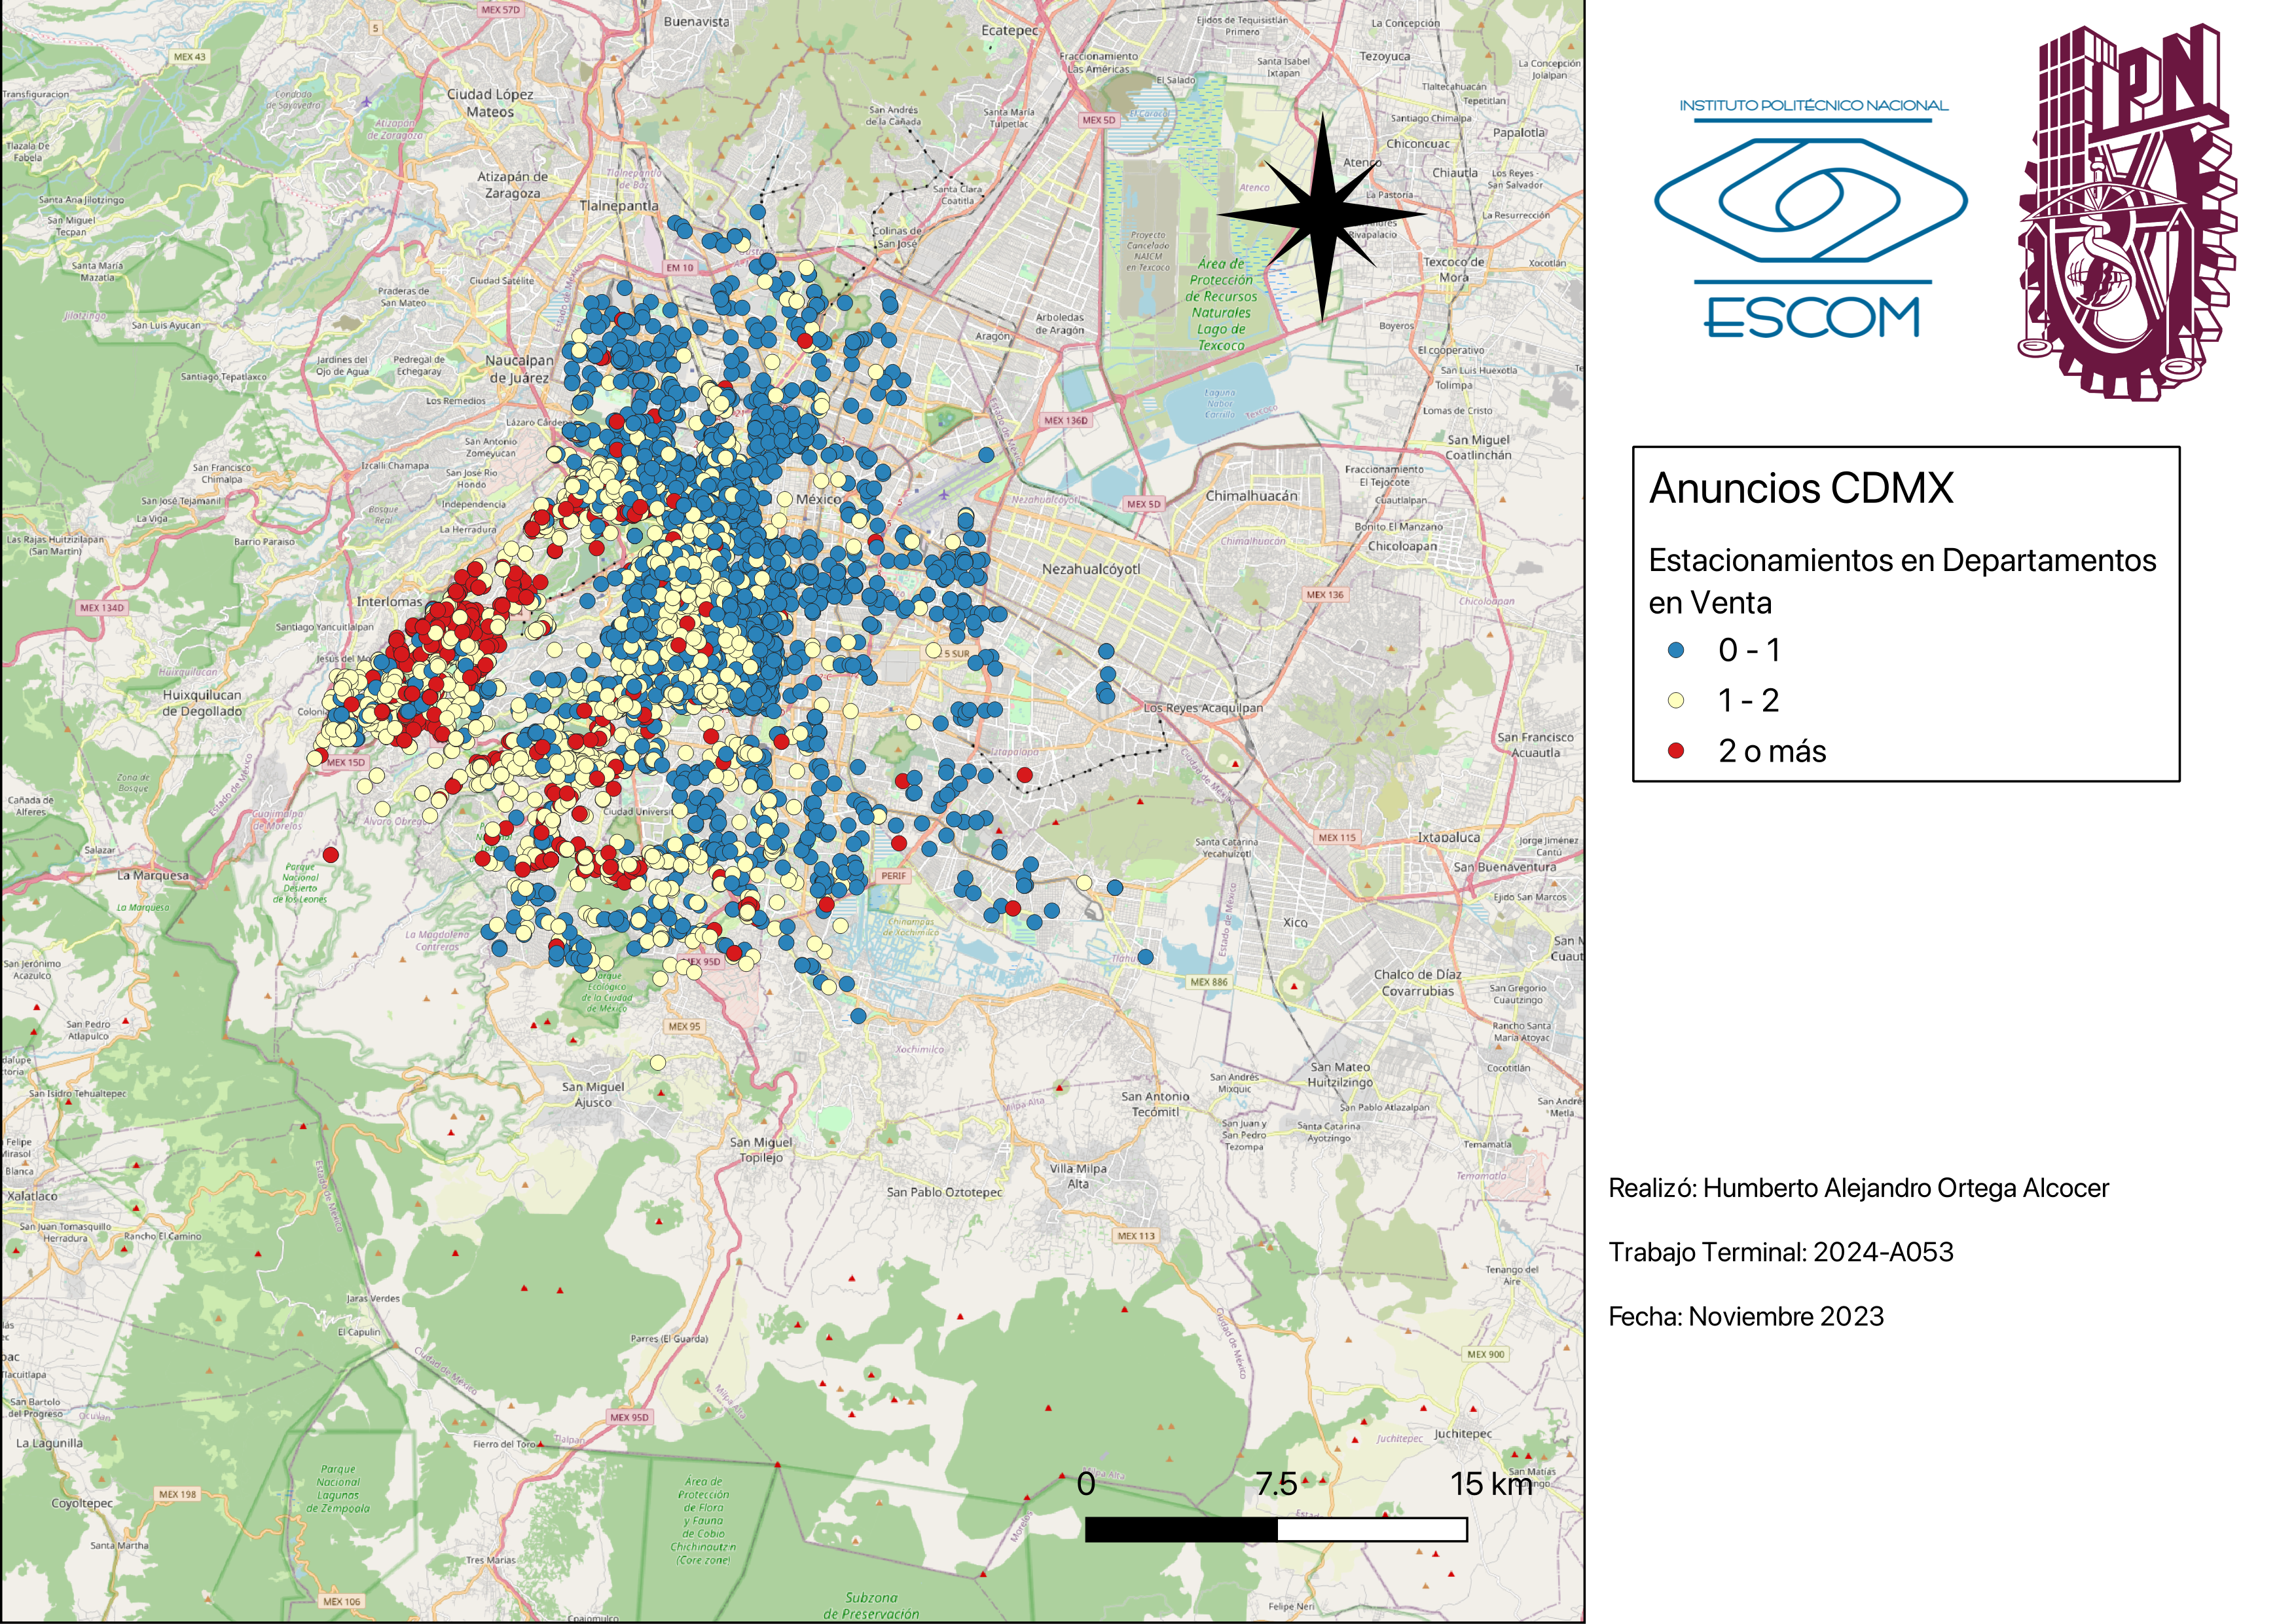
\includegraphics[width=0.9\textwidth]{imagenes/03-analisis/mapa-densidad-estacionamientos.png}
  \caption{Mapa de calor de número de estacionamientos.}
  \label{fig:mapa_calor_estacionamientos}
\end{figure}

De aquí, podemos derivar las siguientes conclusiones:

\begin{itemize}
  \item La gran mayoría de los departamentos en la Ciudad de México tienen 1 o
  2 estacionamientos.
  \item Los departamentos con 1 estacionamiento se encuentran en las zonas con
  mayor densidad de población, como la zona centro de la Ciudad de México.
  \item Los departamentos con 3 o más estacionamientos se encuentran en las
  zonas con mayor precio, como la zona poniene de la Ciudad de México.
\end{itemize}


\subsection{Análisis Exploratorio Econométrico}

La econometría es un campo de estudio que utiliza métodos estadísticos y
matemáticos para analizar y comprender las relaciones económicas, ayudando a
distinguir entre buenas y malas ideas en economía, negocios y políticas
públicas. Se enfoca en proporcionar respuestas cuantitativas a preguntas
importantes en estos ámbitos, permitiendo vislumbrar cómo individuos, empresas
y gobiernos toman decisiones basadas en dichas relaciones. La econometría busca
hacer la teoría inmediatamente relevante para las aplicaciones prácticas,
integrando la teoría y las aplicaciones para hacer el aprendizaje más atractivo
y pertinente \cite{stock2012introduccion}.

El análisis exploratorio econométrico consiste en caracterizar, mediante el uso
de estadísticas descriptivas, las variables que se utilizarán para el
entrenamiento del modelo de aprendizaje automático.

\begin{itemize}
  \item Análisis descriptivo
  \item Correlación entre variables
  \item Análisis de regresión simple y múltiple
  \item Análisis de componentes principales (PCA)
\end{itemize}

\subsubsection{Análisis Descriptivo}

Un análisis descriptivo nos permite caracterizar las variables que se utilizarán
para el entrenamiento del modelo de aprendizaje automático. Además, nos permite
obtener información rápida sobre nuestros datos a bien de poder determinar si
los datos son adecuados para el entrenamiento del modelo.

Para realizar un análisis descriptivo, se utilizó la librería Pandas de Python,
la cual permite realizar análisis descriptivos de manera sencilla. En el Código
\ref{lst:analisis_descriptivo} se muestra el código utilizado para realizar el
análisis descriptivo.

\begin{lstlisting}[language=Python, label=lst:analisis_descriptivo, caption=Análisis descriptivo.]
import pandas as pd

# Carga de datos
df = pd.read_csv('scrape-20231103-16-27-14.csv')

# Columnas a analizar
numeric_columns = ['Price', 'Size_Terrain', 'Size_Construction',
                   'Rooms', 'Bathrooms', 'Parking', 'Age']

# Seleccionar solo las columnas numéricas
df_numeric = df[numeric_columns]

# Analisis descriptivo
resultado = df_numeric.describe(include='all')

# Imprimir resultado
print(resultado)
\end{lstlisting}

En el Cuadro \ref{table:analisis_descriptivo} se muestran los resultados del
análisis descriptivo.

\begin{table}[h!]
\centering
\caption{Estadísticas Descriptivas de los Listados de Bienes Raíces}
\label{table:analisis_descriptivo}
\sisetup{
  round-mode          = places, % Rounds numbers
  round-precision     = 2, % to 2 places
}
\tiny % Makes the font smaller; use \scriptsize or \tiny for even smaller sizes
\begin{tabular}{
  l
  S[table-format=2.2]
  S[table-format=5.0]
  S[table-format=5.0]
  S[table-format=2.0]
  S[table-format=2.0]
  S[table-format=1.0]
  S[table-format=3.0]
}
\toprule
  {} & {Precio (MDP)} & {Superficie} & {Superficie Cons.} & {Recámaras} & {Baños} & {Estacionamiento} & {Antigüedad} \\
\midrule
count & 17.876 & 17740 & 17694 & 17537 & 17478 & 16269 & 10758 \\
mean  & 12.18 & 181 & 156 & 2 & 2 & 2 & 15 \\
std   & 183.45 & 1601 & 426 & 1 & 1 & 1 & 15 \\
min   & 0.0015 & 1 & 1 & 1 & 1 & 1 & 1 \\
25\%  & 3.58 & 75 & 75 & 2 & 2 & 1 & 5 \\
50\%  & 5.65 & 109 & 107 & 2 & 2 & 2 & 10 \\
75\%  & 9.95 & 180 & 179 & 3 & 2 & 2 & 20 \\
max   & 175 & 1401 & 3301 & 6 & 5 & 8 & 310 \\
\bottomrule
\end{tabular}
\normalsize % Resets the font size to normal
\end{table}

De aquí, podemos derivar las siguientes conclusiones:

\begin{itemize}
  \item El precio promedio de las propiedades es de 12.18 millones de pesos, con una amplia variación indicada por una desviación estándar de 183.45 millones de pesos.
  \item La superficie del terreno varía significativamente entre las propiedades, con un promedio de 181 \(m^2\) y una desviación estándar alta de 1601 \(m^2\).
  \item La superficie de construcción promedio es de 155 \(m^2\), con propiedades que van desde 1 \(m^2\) hasta 33015 \(m^2\).
  \item El número promedio de habitaciones por propiedad es de aproximadamente 2.34, con la mayoría de las propiedades teniendo entre 2 y 3 habitaciones.
  \item El número de baños y espacios de estacionamiento también varía, con un promedio cercano a 2 para cada uno.
  \item La edad media de las propiedades es de aproximadamente 14.78 años, con algunas propiedades teniendo hasta 310 años de antigüedad.
  \item Los mínimos en varias categorías (como 1 \(m^2\) de superficie de construcción) podrían indicar datos atípicos o errores en los datos.
\end{itemize}

\subsubsection{Correlación entre variables}

La correlación entre variables nos permite determinar si existe una relación
entre las variables que se utilizarán para el entrenamiento del modelo de
aprendizaje automático. Este análisis es importante ya que nos permite determinar
los pesos que podrían tener las variables en el entrenamiento del modelo. Por
otra parte, entender qué variables tienen más impacto en otras nos permite
determinar si es necesario realizar un análisis de regresión simple o múltiple.

Para realizar un análisis de correlación entre variables, se utilizó la librería
Pandas de Python, la cual permite realizar análisis de correlación entre variables
de manera sencilla. En el Código \ref{lst:correlacion_variables} se muestra el
código utilizado para realizar el análisis de correlación entre variables.

\begin{lstlisting}[language=Python, label=lst:correlacion_variables, caption=Correlación entre variables.]
import pandas as pd

# Carga de datos
df = pd.read_csv('scrape-20231103-16-27-14.csv')

# Columnas a analizar
numeric_columns = ['Price', 'Size_Terrain', 'Size_Construction',
                   'Rooms', 'Bathrooms', 'Parking', 'Age']

# Seleccionar solo columnas numéricas
df_numeric = df[numeric_columns]

# Correlación de Pearson
resultado = df_numeric.corr(method='pearson')

# Imprimir resultado
print(resultado)
\end{lstlisting}

En el Cuadro \ref{table:correlacion_variables} se muestran los resultados del
análisis de correlación entre variables.

\begin{table}[h!]
\centering
\caption{Matriz de Correlación entre Variables}
\label{table:correlacion_variables}
\sisetup{
  round-mode          = places, % Rounds numbers
  round-precision     = 2, % to 2 places
}
\tiny % Makes the font smaller; use \scriptsize or \tiny for even smaller sizes
\begin{tabular}{
  l
  S[table-format=1.2]
  S[table-format=1.2]
  S[table-format=1.2]
  S[table-format=1.2]
  S[table-format=1.2]
  S[table-format=1.2]
  S[table-format=1.2]
}
\toprule
  {} & {Precio} & {Superficie} & {Superficie Cons.} & {Recámaras} & {Baños} & {Estacionamiento} & {Antigüedad} \\
\midrule
Precio              & 1.00 & 0.00 & 0.01 & 0.02 & 0.02 & 0.02 & 0.01 \\
Superficie          & 0.00 & 1.00 & 0.27 & 0.04 & 0.04 & 0.06 & -0.01 \\
Superficie Cons.    & 0.01 & 0.27 & 1.00 & 0.15 & 0.14 & 0.21 & 0.01 \\
Recámaras           & 0.02 & 0.04 & 0.15 & 1.00 & 0.47 & 0.46 & 0.13 \\
Baños               & 0.02 & 0.04 & 0.14 & 0.47 & 1.00 & 0.46 & -0.05 \\
Estacionamiento     & 0.02 & 0.06 & 0.21 & 0.46 & 0.46 & 1.00 & -0.10 \\
Antigüedad          & 0.01 & -0.01 & 0.01 & 0.13 & -0.05 & -0.10 & 1.00 \\
\bottomrule
\end{tabular}
\normalsize % Resets the font size to normal
\end{table}

De aquí, podemos derivar las siguientes conclusiones:

\begin{itemize}
  \item \textbf{Relaciones Débiles}: Los coeficientes de correlación entre el precio y las demás
variables son muy bajos (todos inferiores a 0.03), lo que sugiere que no hay una
relación lineal fuerte entre el precio y las otras características de las
propiedades en el conjunto de datos.
\item \textbf{Superficie y Construcción}: La correlación más fuerte observada es entre la superficie
del terreno y la superficie construida (0.27), lo cual es esperable ya que propiedades
con terrenos más grandes tienden a tener mayores construcciones.
\item \textbf{Recámaras y Baños/Estacionamiento}: Hay una correlación moderada entre el número
de recámaras y baños (0.47) y recámaras y estacionamientos (0.46), lo que indica
que propiedades con más recámaras tienden a tener más baños y más espacio de
estacionamiento.
\item \textbf{Edad de la Propiedad}: La edad tiene una correlación negativa con el estacionamiento
y los baños, aunque es débil. Esto podría sugerir que las propiedades más antiguas
tienen menos baños y menos estacionamientos, pero es una relación muy leve.
\item \textbf{Relevancia para IA}: Para la valuación inmobiliaria con IA utilizando redes
neuronales, estos resultados implican que las variables incluidas no proporcionan
una indicación clara del precio de manera individual. Por lo tanto, el modelo
de red neuronal deberá capturar relaciones no lineales complejas o interacciones
entre variables que no son evidentes a partir de los coeficientes de correlación
lineal.
\end{itemize}

\subsubsection{Análisis de regresión simple y múltiple}

Con el fin de poder determinar la relación entre las variables que se utilizarán
para el entrenamiento del modelo de aprendizaje automático, se realizó un análisis
de regresión simple y múltiple. Las regresiones simples y múltiples son técnicas
estadísticas que permiten determinar la relación entre una variable dependiente
y una o más variables independientes. En el caso de la regresión simple, se
determina la relación entre una variable dependiente y una variable independiente,
mientras que en el caso de la regresión múltiple, se determina la relación entre
una variable dependiente y dos o más variables independientes \cite{stock2012introduccion}.

Para realizar un análisis de regresión simple y múltiple, se utilizó la librería
StatsModels de Python, la cual permite realizar análisis de regresión simple y
múltiple de manera sencilla. En el Código \ref{lst:regresion_simple_multiple} se
muestra el código utilizado para realizar el análisis de regresión simple y múltiple.

\begin{lstlisting}[language=Python, label=lst:regresion_simple_multiple, caption=Regresión simple y múltiple.]
import statsmodels.api as sm
import pandas as pd
import numpy as np

# Carga de datos
df = pd.read_csv('scrape-20231103-16-27-14.csv')

# Reemplazar infinitos con NaN
df.replace([np.inf, -np.inf], np.nan, inplace=True)

# Eliminar filas con valores NaN
df_clean = df.dropna(subset=['Price','Size_Terrain', 'Size_Construction',
                             'Rooms', 'Bathrooms', 'Parking'])

# Columnas a analizar
numeric_columns = ['Price', 'Size_Terrain', 'Size_Construction',
                   'Rooms', 'Bathrooms', 'Parking', 'Age']

# Seleccionar solamente columnas numéricas
df_numeric = df_clean[numeric_columns]

# Regresión simple usando Size_Construction como predictor del Price
X_simple = sm.add_constant(df_numeric['Size_Construction']) # Añadir constante
modelo_simple = sm.OLS(df_numeric['Price'], X_simple).fit()

# Regresión múltiple usando Size_Construction, Rooms, Bathrooms y Parking como predictores del Price
X_multiple = sm.add_constant(df_numeric[['Size_Terrain', 'Rooms', 'Bathrooms', 'Parking']]) # Añadir constante
modelo_multiple = sm.OLS(df_numeric['Price'], X_multiple).fit()

# Imprimir los resultados
print("Regresión simple")
print(modelo_simple.summary())
print()
print("Regresión múltiple")
print(modelo_multiple.summary())
\end{lstlisting}

En el Cuadro \ref{table:regresion_simple} se muestran los resultados del análisis
de regresión simple.

\begin{table}[ht!]
\centering
\caption{Resultados de la Regresión Simple}
\label{table:regresion_simple}
\begin{tabular}{
  l
  S[table-format=-1.4]
  S[table-format=1.4]
}
\toprule
{Variable} & {Coeficiente} & {Error Estándar} \\
\midrule
Constante              & 1.21e+07 & 1.69e+06 \\
Size\_Construction & 4917.3102 & 4216.805 \\
\bottomrule
\end{tabular}
\end{table}

\textit{Nota:} R-cuadrado: 0.000; F-estadístico: 1.360, P-valor: 0.244. El Omnibus y Jarque-Bera indican una distribución no normal de los residuos.

En el Cuadro \ref{table:regresion_multiple} se muestran los resultados del análisis
de regresión múltiple.

\begin{table}[h!]
\centering
\caption{Resultados de la Regresión Múltiple}
\label{table:regresion_multiple}
\begin{tabular}{
  l
  S[table-format=-1.4]
  S[table-format=1.4]
}
\toprule
{Variable} & {Coeficiente} & {Error Estándar} \\
\midrule
Constante         & -6.191e+04 & 5.63e+06 \\
Size\_Terrain     & 76.1953    & 925.533 \\
Rooms             & 1.772e+06  & 2.6e+06 \\
Bathrooms         & 1.304e+06  & 1.8e+06 \\
Parking           & 3.122e+06  & 2.03e+06 \\
\bottomrule
\end{tabular}
\end{table}

\textit{Nota:} R-cuadrado: 0.001; F-estadístico: 2.021, P-valor: 0.0887. Las notas adicionales mencionan errores estándar que asumen que la matriz de covarianza de los errores está correctamente especificada y un número de condición grande, lo que podría indicar multicolinealidad.

De los resultados obtenidos, podemos derivar las siguientes conclusiones:

\begin{itemize}
  \item Para la regresión simple, el R-cuadrado es 0, lo que indica que el modelo
    no explica nada de la variabilidad del precio. Esto está reforzado por el alto
    P-valor, sugiriendo que la variable Size\_Construction no es un predictor
    estadísticamente significativo del precio.
  \item Para la regresión múltiple, aunque incluye más variables, el R-cuadrado
    sigue siendo muy bajo (0.001), indicando que el modelo explica menos del 0.1\%
    de la variabilidad del precio. Los P-valores también son altos, sugiriendo
    que ninguna de las variables independientes es un predictor significativo
    del precio.
  \item Las altas estadísticas de Omnibus y Jarque-Bera junto con la significativa
    desviación (skewness) y la kurtosis apuntan a una distribución no normal de los
    residuos, lo que podría afectar la fiabilidad de los tests estadísticos.
  \item El número de condición alto en la regresión múltiple sugiere que podría
    haber problemas de multicolinealidad en el modelo, lo que significa que
    algunas de las variables independientes están correlacionadas entre sí.
\end{itemize}

\subsubsection{Análisis de componentes principales (PCA)}

El análisis de componentes principales es un método estadístico versátil para
reducir una tabla de datos de casos por variables a sus características esenciales,
llamadas componentes principales. Los componentes principales son unas pocas
combinaciones lineales de las variables originales que explican de manera
máxima la varianza de todas las variables. En el proceso, el método proporciona
una aproximación de la tabla de datos original utilizando solo estos pocos
componentes principales \cite{greenacre2022principal}.

Para poder llevar a cabo este análisis, se utilizó la librería Scikit-Learn de
Python, la cual permite realizar análisis de componentes principales de manera
sencilla. En el Código \ref{lst:pca} se muestra el código utilizado para realizar
el análisis de componentes principales.

\begin{lstlisting}[language=Python, label=lst:pca, caption=Análisis de componentes principales (PCA).]
import pandas as pd
import numpy as np
from sklearn.decomposition import PCA
from sklearn.preprocessing import StandardScaler

# Carga de datos
df = pd.read_csv('scrape-20231103-16-27-14.csv')

# Reemplazar infinitos con NaN
df.replace([np.inf, -np.inf], np.nan, inplace=True)

# Eliminar filas con valores NaN
df_clean = df.dropna(subset=['Price','Size_Terrain', 'Size_Construction',
                             'Rooms', 'Bathrooms', 'Parking', 'Age'])

# Columnas a analizar
numeric_columns = ['Price', 'Size_Terrain', 'Size_Construction',
                   'Rooms', 'Bathrooms', 'Parking', 'Age']

# Seleccionar únicamente las columnas numéricas
df_numeric = df_clean[numeric_columns]

# Estandarizar los datos
scaler = StandardScaler()
df_scaled = scaler.fit_transform(df_numeric)

# PCA
pca = PCA(n_components=2) # Reducir a 2 componentes principales

componentes_principales = pca.fit_transform(df_scaled)

# Imprimir los componentes principales
print('Componentes principales')
print(componentes_principales)

# Varianza explicada
print('Varianza explicada')
print(pca.explained_variance_ratio_)

# Coeficientes de los componentes
print('Coeficientes de los componentes')
print(pca.components_)


\end{lstlisting}

Los resultados del análisis de componentes principales se muestran en el Cuadro
\ref{table:pca-results}.

\begin{table}[h]
\small
\centering
\begin{tabular}{|c|c|c|}
\hline
\rowcolor{azulclaro}
  \textbf{Componente} & \textbf{Varianza Explicada} & \textbf{Coeficientes} \\ \hline
1 & 30.61\% & [0.047, 0.083, 0.458, 0.505, 0.485, 0.537, 0.051] \\ \hline
2 & 15.42\% & [0.185, -0.094, 0.008, 0.255, -0.109, -0.237, 0.908] \\ \hline
\end{tabular}
\caption{Resultados del Análisis de Componentes Principales}
\label{table:pca-results}
\end{table}

En la figura \ref{fig:pca} se muestra la visualización de los componentes
principales.

\begin{figure}[H]
  \centering
  \includegraphics[width=0.8\textwidth]{imagenes/03-analisis/analisis-econometrico/analisis-pca.png}
  \caption{Visualización de los componentes principales.}
  \label{fig:pca}
\end{figure}

De los resultados obtenidos, podemos derivar las siguientes conclusiones:

\begin{enumerate}
    \item Las características físicas de los inmuebles, como el tamaño de la construcción, el número de habitaciones, baños y estacionamientos, son las que más varían y tienen mayor influencia en el primer componente principal.
    \item La edad del inmueble es una dimensión importante de variabilidad y es el factor predominante en el segundo componente principal.
    \item Estos dos componentes capturan casi la mitad de la variabilidad total de los datos, lo que indica una distribución equilibrada de la influencia de las diferentes variables.
    \item Se recomienda visualizar estos componentes principales en un gráfico bidimensional para identificar patrones o agrupaciones interesantes en los datos.
    \item Dependiendo de los objetivos del análisis, podría ser útil considerar aumentar el número de componentes principales para capturar más variabilidad.
\end{enumerate}

\section{Algoritmos de Aprendizaje Automático}

Para la realización de este proyecto se deberán considerar múltiples algoritmos
de aprendizaje automático, los cuales se utilizarán para el entrenamiento de los
modelos de valuación inmobiliaria. Estos algoritmos serán utilizados para realizar
una comparativa entre el rendimiento y ajuste de cada uno con el objetivo de
poder determinar, una vez finalizada la creación del conjunto de datos final,
cuál algoritmo emplear para la creación del modelo de valuación inmobiliaria final.

\subsection{Máquinas de Soporte Vectorial}

Método efectivo en espacios de alta dimensión. Utiliza hiperplanos para separar
clases de datos. Los hiperplanos se eligen maximizando el margen entre las clases.
Las SVMs pueden usar diferentes tipos de kernels, como lineal, polinomial y
radial, para adaptarse a la naturaleza no lineal de algunos datos \cite{10.1145/1143844.1143865}.

\subsection{Random Forest}

El algoritmo de bosques aleatorios, propuesto por L. Breiman en 2001, ha
sido extremadamente exitoso como un método de clasificación y regresión de propósito
general. El enfoque, que combina varios árboles de decisión aleatorizados y
agrega sus predicciones mediante promedios, ha mostrado
un excelente rendimiento en entornos donde el número de variables es
mucho mayor que el número de observaciones. Además, es lo suficientemente versátil
como para ser aplicado a problemas a gran escala, se adapta fácilmente a
varias tareas de aprendizaje ad hoc y devuelve medidas de la importancia de las variables
\cite{biau2016random}.

\subsection{Redes Neuronales Artificiales}

Las redes neuronales son un modelo de aprendizaje automático inspirado en el
funcionamiento del cerebro humano. Las redes neuronales se componen de neuronas
artificiales que se conectan entre sí para formar una red. Cada neurona artificial
tiene una o más entradas y una salida. Las entradas de una neurona artificial
están conectadas a otras neuronas artificiales a través de conexiones llamadas
pesos. Cada conexión tiene un peso asociado con él. El peso de una conexión
determina la influencia de una neurona en otra. Las neuronas artificiales
utilizan una función de activación para determinar su salida en función de sus
entradas y pesos. Las redes neuronales se utilizan para resolver problemas de
clasificación y regresión \cite{muller1995neural}.

\section{Estudio de Factibilidad}

Para poder determinar si el proyecto es factible, se realizó un estudio de
factibilidad, el cual se divide en tres partes: factibilidad técnica, factibilidad
económica y factibilidad operativa.

El objetivo general será determinar si el planteamiento del proyecto es viable
y si se puede llevar a cabo con los recursos disponibles.

\subsection{Factibilidad Técnica}

En el apartado de factibilidad técnica se analizaron los recursos técnicos
necesarios para poder llevar a cabo el proyecto planteado en el presente
documento. En el Cuadro \ref{table:factibilidad_tecnica} se muestra el análisis
de factibilidad técnica.

\begin{table}[H]
\centering
\begin{tabular}{|p{5cm}|c|c|}
\hline
\rowcolor{azulclaro}
  \centering\textbf{Recurso} & \centering\textbf{Disponibilidad}\arraybackslash & \centering\textbf{Viabilidad}\arraybackslash \\
\hline
Equipo de cómputo & Sí & Sí \\
\hline
  Software & Sí & Sí \\
\hline
  Conexión a internet & Sí & Sí \\
\hline
  Plataforma en la nube & Sí & Sí \\
\hline
\end{tabular}
\caption{Factibilidad Técnica}
\label{table:factibilidad_tecnica}
\end{table}

Dado que todos los recursos necesarios para llevar a cabo el proyecto se
encuentran disponibles, se puede concluir que el proyecto es factible desde el
punto de vista técnico.

\subsection{Factibilidad Económica}

Para llevar a cabo el proyecto será necesario contar con un presupuesto, el cual
se utilizará para la adquisición de recursos necesarios para el desarrollo del
mismo. En el Cuadro \ref{table:factibilidad_economica} se muestra el análisis de
factibilidad económica.

\begin{table}[H]
\centering
\begin{tabular}{|p{5cm}|c|c|}
\hline
\rowcolor{azulclaro}
  \centering\textbf{Recurso} & \textbf{Costo} & \textbf{Viabilidad}\arraybackslash \\
\hline
AWS & \$ 10 USD/mes & Sí \\
\hline
Equipo de cómputo & \$ 20,000.00 & Sí \\
\hline
  Recursos Humanos & \$ 15,000.00/mes & Sí \\
\hline
\end{tabular}
\caption{Factibilidad Económica}
\label{table:factibilidad_economica}
\end{table}

\textit{*Nota:} AWS ofrece un plan gratuito que incluye 750 horas de uso de instancias EC2
t2.micro, 5 GB de almacenamiento EBS, 40 GB de almacenamiento EFS, 750 horas de
uso de RDS, 25 horas de uso de DynamoDB, 15 GB de ancho de banda de salida, 1
millón de solicitudes de Lambda y 1 millón de solicitudes de API Gateway al mes
durante un año \cite{aws_free_2023}. A pesar de esto, se incluyó el costo de AWS
en el análisis de factibilidad económica para poder tener un presupuesto más realista
e inclusive realizar las proyecciones pertinentes en caso de que se requiera
utilizar recursos adicionales a los ofrecidos en el plan gratuito.

Debido a que se estiman 6 meses de trabajo, los costos finales del proyecto
se observan en el Cuadro \ref{table:costos_proyecto}.

\begin{table}[H]
\centering
\begin{tabular}{|c|p{5cm}|}
\hline
\rowcolor{azulclaro}
  \textbf{Recurso} & \centering\textbf{Costo}\arraybackslash \\
\hline
  AWS & \$ 60 USD (~\$1,029.00 MN) \\
\hline
Equipo de cómputo & \$20,000.00 MN\\
\hline
  Recursos Humanos & \$90,000.00 MN \\
\hline
\textbf{Costo Total} & \textbf{\$ 111,060.00 MN} \\
\hline
\end{tabular}
\caption{Costos del Proyecto (6 meses) en Moneda Nacional}
\label{table:costos_proyecto}
\end{table}

Dado que el costo total del proyecto es de \$111,060.00 MN y que se cuenta con
un presupuesto de \$150,000.00 MN, se puede concluir que el proyecto es factible
desde el punto de vista económico y contempla un margen de \$38,940.00 MN para
gastos adicionales.

\subsection{Factibilidad Operativa}

Debido a que el proyecto se realizará en un periodo de 6 meses, se debe
contar con el tiempo suficiente para llevar a cabo cada una de las tareas, al
igual que el equipo de trabajo deberá conocer las herramientas a utilizar para
el desarrollo del proyecto. En el Cuadro \ref{table:factibilidad_operativa} se
muestra el análisis de factibilidad operativa.

\begin{table}[H]
\centering
\begin{tabular}{|p{5cm}|c|c|}
\hline
\rowcolor{azulclaro}
  \centering\textbf{Recurso} & \centering\textbf{Disponibilidad}\arraybackslash & \centering\textbf{Viabilidad}\arraybackslash \\
\hline
Tiempo & Sí & Sí \\
\hline
  Equipo de trabajo & Sí & Sí \\
\hline
Conocimiento & Sí & Sí \\
\hline
\end{tabular}
\caption{Factibilidad Operativa}
\label{table:factibilidad_operativa}
\end{table}

Dado que se cuenta con el tiempo necesario para llevar a cabo el proyecto, se
cuenta con el equipo de trabajo y dicho equipo cuenta con el conocimiento para
desarrollar el proyecto, se puede concluir que el proyecto es factible desde el
punto de vista operativo.

\subsection{Factibilidad General}

Dado que el proyecto es factible desde el punto de vista técnico, económico y
operativo, podemos concluir que el proyecto es \textit{factible} y se puede
llevar a cabo con los recursos disponibles.

\subsection{Consideraciones Legales}

Los datos que se utilizarán para el desarrollo del proyecto son datos obtenidos
de distintas plataformas online de bienes raíces, por lo que se debe tener en
cuenta las políticas de privacidad de cada una de las plataformas para poder
utilizar los datos de manera adecuada.

En México, la \acrfull{lfpdppp} es la ley que regula el tratamiento de los datos
personales en posesión de los particulares, con el fin de regular su uso,
conservación y transferencia \cite{dof2010lfpdppp}.

Dado que no se utilizarán datos personales para el desarrollo del proyecto, no
se deberá tener ningún problema con la \acrshort{lfpdppp}. Sin embargo, y debido a que los
datos iniciales (sin preprocesamiento) contienen los campos de ``Descripción'' y ``Título'' del anuncio (los cuales
son campos abiertos y podrían contener información sensible), se debe de tener
presente esta ley para descartar el uso de dichos campos en el entrenamiento del modelo.

\section{Análisis de Riesgos}

Todo proyecto conlleva riesgos, los cuales pueden afectar el desarrollo del
mismo. A bien de poder realizar una planeación apropiada del proyecto a llevar
a cabo, se realizó un análisis de riesgos, en el cual se identificaron los
riesgos más importantes que pueden afectar el desarrollo del proyecto. Para cada
uno de los riesgos identificados, se utilizó una matriz de riesgos como se puede
observar en la Figura \ref{fig:matriz_riesgos_inicial}.

\begin{figure}[H]
  \centering
  \includegraphics[width=0.8\textwidth]{imagenes/03-analisis/analisis-riesgos/matriz-riesgos-inicial.png}
  \caption{Matriz de riesgos inicial.}
  \label{fig:matriz_riesgos_inicial}
\end{figure}

En esta matriz se pueden visualizar tres parámetros importantes para cada riesgo:

\begin{itemize}
  \item \textbf{Impacto:} El impacto que tendrá el riesgo en el proyecto, el cual
  se encuentra en una escala de 1 a 5, donde 1 es el impacto más bajo y 5 es el
  impacto más alto.
  \item \textbf{Probabilidad:} La probabilidad de que el riesgo ocurra, la cual
  se encuentra en una escala de 1 a 5, donde 1 es la probabilidad más baja y 5 es
  la probabilidad más alta.
  \item \textbf{Advertencia Avanzada:} El tiempo de advertencia que se tiene
  antes de que el riesgo ocurra, la cual se encuentra en una escala de 1 a 5,
  dónde 1 representa un riesgo totalmente desconocido y 5 representa un riesgo
  que se puede predecir con mucha anticipación.
\end{itemize}

Con estos tres parámetros se puede calcular el nivel de riesgo de cada riesgo
identificado, el cual, por su ubicación en la matriz, se puede clasificar en
bajo, medio o alto. Con esta información se puede realizar una planeación
apropiada para cada riesgo, con el fin de mitigar el impacto que este pueda
tener en el proyecto.

\subsection{Riesgo de Cronograma}

Si se realizó una mala estimación sobre el tiempo que tomará la realización del
presente proyecto o si surgió una afectación a algún recurso, sea o no humano,
se puede presentar un retraso en la entrega del proyecto. En el Cuadro
\ref{table:riesgo_cronograma} se muestra el riesgo de cronograma.

\begin{table}[H]
\centering
\begin{tabular}{|c|p{5cm}|c|}
\hline
\rowcolor{azulclaro}
  \centering\textbf{Impacto} & \centering\textbf{Advertencia Avanzada}\arraybackslash & \centering\textbf{Probabilidad}\arraybackslash \\
\hline
  Medio (3) & Conocido - informado, documentado (5) & Baja (1) \\
\hline
\end{tabular}
\caption{Riesgo de Cronograma}
\label{table:riesgo_cronograma}
\end{table}

En la Figura \ref{fig:riesgo_cronograma} se muestra la ubicación del riesgo de
cronograma en la matriz de riesgos.

\begin{figure}[H]
  \centering
  \includegraphics[width=0.8\textwidth]{imagenes/03-analisis/analisis-riesgos/riesgo-cronograma.png}
  \caption{Matriz de riesgo de cronograma.}
  \label{fig:riesgo_cronograma}
\end{figure}

\subsubsection{Mitigación de los riesgos de cronograma}

Para mitigar el riesgo de cronograma, se realizará una planeación adecuada de
las tareas a realizar, con el fin de poder realizar una estimación adecuada del
tiempo que tomará cada una de las tareas. Por otra parte, se realizará un
seguimiento constante del avance del proyecto, con el fin de poder detectar
cualquier retraso en el cronograma y poder tomar las acciones necesarias para
poder cumplir con los tiempos establecidos.

A su vez, se asignarán las tareas con tiempo de sobra para poder cumplir con
los tiempos establecidos, con el fin de poder tener un margen de error en caso
de que se presente algún retraso en el cronograma.

\subsection{Riesgo de Costos}

Si se llegara a rebasar el límite de presupuesto asignado para el proyecto, se
puede presentar un retraso en la entrega del proyecto. En el Cuadro
\ref{table:riesgo_costos} se muestra el riesgo de costos.

\begin{table}[H]
\centering
\begin{tabular}{|c|p{5cm}|c|}
\hline
\rowcolor{azulclaro}
  \centering\textbf{Impacto} & \centering\textbf{Advertencia Avanzada}\arraybackslash & \centering\textbf{Probabilidad}\arraybackslash \\
\hline
  Medio Alto (4) & Conocido - no informado, no documentado (2) & Media (2) \\
\hline
\end{tabular}
\caption{Riesgo de Costos}
\label{table:riesgo_costos}
\end{table}

En la Figura \ref{fig:riesgo_costos} se muestra la ubicación del riesgo de
costos en la matriz de riesgos.

\begin{figure}[H]
  \centering
  \includegraphics[width=0.8\textwidth]{imagenes/03-analisis/analisis-riesgos/riesgo-costos.png}
  \caption{Matriz de riesgo de costos.}
  \label{fig:riesgo_costos}
\end{figure}

\subsubsection{Mitigación de los riesgos de costos}

Para prevenir que excedamos el presupuesto del proyecto, o que se presenten
costos no contemplados en el presupuesto, se realizará una planeación adecuada
de los recursos necesarios para el desarrollo del proyecto, con el fin de poder
contar con un presupuesto adecuado para el desarrollo del proyecto. Igualmente,
se realizará la planeación considerando un margen de error, con el fin de poder
disponer de recursos adicionales en caso de que se presenten costos no contemplados.

\subsection{Riesgo Tecnológico}

En caso de que se presenten cambios en las tecnologías seleccionadas para el
proyecto, o si hubiese un cambio en las herramientas de desarrollo, o en los
datos disponibles para el entrenamiento del modelo, se puede presentar un
retraso en la entrega del proyecto. En el Cuadro \ref{table:riesgo_tecnologico}
se muestra el riesgo tecnológico.

\begin{table}[H]
\centering
\begin{tabular}{|c|p{5cm}|c|}
\hline
\rowcolor{azulclaro}
  \centering\textbf{Impacto} & \centering\textbf{Advertencia Avanzada} & \centering\textbf{Probabilidad}\arraybackslash \\
\hline
  Medio Alto (4) & Conocido - no informado, documentado (3) & Alta (3) \\
\hline
\end{tabular}
\caption{Riesgo Tecnológico}
\label{table:riesgo_tecnologico}
\end{table}

En la Figura \ref{fig:riesgo_tecnologico} se muestra la ubicación del riesgo
tecnológico en la matriz de riesgos.

\begin{figure}[H]
  \centering
  \includegraphics[width=0.8\textwidth]{imagenes/03-analisis/analisis-riesgos/riesgo-tecnologico.png}
  \caption{Matriz de riesgo tecnológico.}
  \label{fig:riesgo_tecnologico}
\end{figure}

\subsubsection{Mitigación de los riesgos tecnológicos}

Para mitigar el riesgo tecnológico, se realizará una investigación adecuada de
las tecnologías a utilizar, con el fin de poder seleccionar las tecnologías más
adecuadas para el desarrollo del proyecto. Se considerarán las aptitudes y
conocimientos del equipo de trabajo, así como la documentación disponible para
cada una de las tecnologías a utilizar.

\subsection{Riesgo Operacional}

Al ser un proyecto que puede prestarse a muchos criterios sobre las conclusiones
que pudiesen derivarse sobre los datos empleados para el mismo, se puede
presentar un riesgo operacional. Esto puede presentarse tanto en falta de
aptitudes del equipo de trabajo, falta de conocimiento sobre el tema, o falta
de conocimiento sobre las herramientas empleadas. En el Cuadro
\ref{table:riesgo_operacional} se muestra el riesgo operacional.

\begin{table}[H]
\centering
\begin{tabular}{|c|p{5cm}|c|}
\hline
\rowcolor{azulclaro}
  \centering\textbf{Impacto} & \centering\textbf{Advertencia Avanzada}\arraybackslash & \centering\textbf{Probabilidad}\arraybackslash \\
\hline
  Medio (3) & Conocido - informado, no documentado (4) & Media (2) \\
\hline
\end{tabular}
\caption{Riesgo Operacional}
\label{table:riesgo_operacional}
\end{table}

En la Figura \ref{fig:riesgo_operacional} se muestra la ubicación del riesgo
operacional en la matriz de riesgos.

\begin{figure}[H]
  \centering
  \includegraphics[width=0.8\textwidth]{imagenes/03-analisis/analisis-riesgos/riesgo-operacional.png}
  \caption{Matriz de riesgo operacional.}
  \label{fig:riesgo_operacional}
\end{figure}

\subsubsection{Mitigación de los riesgos operacionales}

Para mitigar el riesgo operacional, se realizará una investigación adecuada de
las conclusiones que se puedan derivar de los datos, con el fin de poder
delimitar y documentar aquellas que resulten más relevantes para el proyecto.

\subsection{Riesgos Externos}

Si las plataformas en la nube descontinuaran algún servicio utilizado para el
alojamiento, procesamiento o análisis de datos, se puede presentar un retraso
en la entrega del proyecto. En el Cuadro \ref{table:riesgo_externo} se muestra
el riesgo externo.

\begin{table}[H]
\centering
\begin{tabular}{|c|p{5cm}|c|}
\hline
\rowcolor{azulclaro}
  \centering\textbf{Impacto} & \centering\textbf{Advertencia Avanzada}\arraybackslash & \centering\textbf{Probabilidad}\arraybackslash \\
\hline
  Medio Alto (4) & Conocido - informado, no documentado (4) & Baja (1) \\
\hline
\end{tabular}
\caption{Riesgo Externo}
\label{table:riesgo_externo}
\end{table}

En la Figura \ref{fig:riesgo_externo} se muestra la ubicación del riesgo
externo en la matriz de riesgos.

\begin{figure}[H]
  \centering
  \includegraphics[width=0.8\textwidth]{imagenes/03-analisis/analisis-riesgos/riesgo-externo.png}
  \caption{Matriz de riesgo externo.}
  \label{fig:riesgo_externo}
\end{figure}

\subsubsection{Mitigación de los riesgos externos}

Para prevenir que algún actor o factor externo pudiese afectar en el desarrollo
del proyecto, se realizará una investigación adecuada de las plataformas en la
nube a utilizar, con el fin de poder seleccionar aquellas que sean más estables
así como los servicios que ofrezcan, con el fin de poder evitar que se presenten
cambios en los servicios que puedan afectar el desarrollo del proyecto.

\subsection{Riesgos Legales}

Si se llegara a presentar un cambio en las leyes que regulan el uso de los datos
empleados para el entrenamiento del modelo, se puede presentar un retraso en la
entrega del proyecto. En el Cuadro \ref{table:riesgo_legal} se muestra el riesgo
legal.

\begin{table}[H]
\centering
\begin{tabular}{|c|p{5cm}|c|}
\hline
\rowcolor{azulclaro}
  \centering\textbf{Impacto} & \centering\textbf{Advertencia Avanzada}\arraybackslash & \centering\textbf{Probabilidad}\arraybackslash \\
\hline
  Bajo (2) & Conocido - informado, documentado (5) & Baja (1) \\
\hline
\end{tabular}
\caption{Riesgo Legal}
\label{table:riesgo_legal}
\end{table}

En la Figura \ref{fig:riesgo_legal} se muestra la ubicación del riesgo legal
en la matriz de riesgos.

\begin{figure}[H]
  \centering
  \includegraphics[width=0.8\textwidth]{imagenes/03-analisis/analisis-riesgos/riesgo-legal.png}
  \caption{Matriz de riesgo legal.}
  \label{fig:riesgo_legal}
\end{figure}

\subsubsection{Mitigación de los riesgos legales}

Gracias a la realización del estudio de factibilidad, se pudo determinar que
no se utilizarán datos personales para el desarrollo del proyecto, por lo que
no se deberá tener ningún problema con la \acrfull{lfpdppp}. Sin embargo, y debido a que
los datos iniciales (sin preprocesamiento) contienen los campos de ``Descripción'' y ``Título''' del anuncio (los cuales
son campos abiertos y podrían contener información sensible), se debe de tener
presente esta ley para descartar el uso de dichos campos en el entrenamiento del modelo.

\subsection{Riesgos generalizados}

En la Figura \ref{fig:riesgos_generalizados} se muestra la ubicación de cada
uno de los riesgos descritos anteriormente a bien de poder visualizarlos en
conjunto.

\begin{figure}[H]
  \centering
  \includegraphics[width=0.8\textwidth]{imagenes/03-analisis/analisis-riesgos/riesgos-generalizados.png}
  \caption{Matriz de riesgos generalizados.}
  \label{fig:riesgos_generalizados}
\end{figure}

\subsection{Exposición al Riesgo}

En la Figura \ref{fig:exposicion_riesgo} se muestra la exposición al riesgo de
cada uno de los riesgos descritos anteriormente a bien de poder tener una idea
de con cuales riesgos se deberá tener más precaución durante el desarrollo
del proyecto.

\begin{figure}[H]
  \centering
  \includegraphics[width=0.8\textwidth]{imagenes/03-analisis/analisis-riesgos/exposicion-riesgos.png}
  \caption{Exposición al riesgo.}
  \label{fig:exposicion_riesgo}
\end{figure}

Debido a que el proyecto se encuentra mayoritariamente expuesto al riesgo
tecnológico de costos, se tendrá especial cuidado con los aspectos de selección
de herramientas tecnológicas y de planeación de costos. Por otra parte, se
preferirá utilizar herramientas de código abierto para evitar costos de licencias
y cambios abruptos en las herramientas utilizadas.
